%!TEX encoding = UTF-8 Unicode
\documentclass{ctexart}
\usepackage{color}
\usepackage{xcolor}
\usepackage{amsmath}
\usepackage{amssymb}
\usepackage{esint}
\usepackage{graphicx}
\usepackage{bm}
\usepackage{multirow}

\numberwithin{equation}{section}

\newtheorem{Definition}{\hspace{2em}定义}
\newtheorem{theorem}{\hspace{2em}定理}
\newtheorem{lemma}{\hspace{2em}引理}
\newtheorem{Proof}{证明}
\newtheorem{remark}{注}
\newtheorem{example}{例子}

\colorlet{RED}{red}

\begin{document}

\title{大规模并行处理器编程-实践方法}

\author{杨丰}
\date{}
\maketitle

\tableofcontents

\newpage
\section*{推荐序}
Wen-mei 和 David 的《大规模并行处理器编程》(第四版)由两位杰出的计算机科学家和 GPU 计算先驱撰写,
作者为 Wen-mei W. Hwu、David B. Kirk 和 Izzat El Hajj,继续为该领域做出了宝贵贡献。 创建新的计算模型。

GPU 计算已成为现代科学的重要工具。 本书将教您如何使用该仪器,并为您提供解决最具挑战性问题的超强工具。 
GPU 计算将成为一台让您看到未来的时间机器,一艘带您前往触手可及的新世界的宇宙飞船。

解决世界上许多最具影响力的问题都需要计算性能。 从计算机历史的开始,架构师就寻求并行计算技术来提高性能。 
一百倍的提升相当于依赖顺序处理的 CPU 进步了十年。 尽管并行计算有巨大的好处,
但创建一个用户、开发者、供应商和分销商良性循环的新计算模型一直是一个令人畏惧的先有鸡还是先有蛋的问题。

近三十年后,NVIDIA GPU 计算已经普及,数百万开发人员已经学习了并行编程,其中许多是从本书的早期版本中学习的。

GPU 计算正在影响科学和工业的各个领域,甚至计算机科学本身。 GPU 的处理速度使深度学习模型能够从数据中学习并执行智能任务,
掀起了从自动驾驶车辆、机器人到合成生物学的发明浪潮。 人工智能时代正在到来。

人工智能甚至正在学习物理学,并开启了以比以往快一百万倍的速度模拟地球气候的可能性。 
NVIDIA 正在构建一款名为 Earth-2 的 GPU 超级计算机(地球的数字孪生),
并与世界科学界合作,预测当今的行为对数十年后气候的影响。

一位生命科学研究人员曾经对我说:“因为有了你的 GPU,我可以在有生之年完成我一生的工作。” 
因此,无论您是在推进人工智能还是在进行突破性科学,我希望 GPU 计算能够帮助您完成您一生的工作。
\\
\rightline{黄仁勋}

\newpage
\section*{前言}
我们很自豪地向您介绍第四版《大规模并行处理器编程:实践方法》。

结合了多核 CPU 和多线程 GPU 的大众市场计算系统为笔记本电脑带来了万亿级计算,为集群带来了百亿亿级计算。 
有了这样的计算能力,我们正处于科学、工程、医学和商业学科中广泛使用计算实验的黎明。 
我们还见证了 GPU 计算在金融、电子商务、石油和天然气以及制造等关键行业垂直市场中的广泛采用。 
这些学科的突破将通过使用规模、准确性、安全性、可控性和可观察性达到前所未有的水平的计算实验来实现。 
本书为这一愿景提供了一个关键要素:向数百万研究生和本科生教授并行编程,以便计算思维和并行编程技能将像微积分技能一样普及。

本书的主要目标读者包括所有科学和工程学科的研究生和本科生,这些学科需要计算思维和并行编程技能才能取得突破。 
本书还被需要更新并行计算技能并跟上不断增长的技术发展速度的行业专业开发人员成功使用。 
这些专业开发人员的工作领域包括机器学习、网络安全、自动驾驶汽车、计算金融、数据分析、认知计算、机械工程、
土木工程、电气工程、生物工程、物理、化学、天文学和地理学,他们使用计算 来推进他们的领域。 
因此,这些开发人员既是各自领域的专家,又是程序员。 本书采用通过建立对技术的直观理解来教授并行编程的方法。 
我们假设读者至少有一些基本的 C 编程经验。 我们使用 CUDA C,这是 NVIDIA GPU 支持的并行编程环境。 
消费者和专业人士手中有超过 10 亿个这样的处理器,超过 40 万程序员正在积极使用 CUDA。 
作为学习体验的一部分,您将开发的应用程序将可由非常大的用户社区运行。

自2016年第三版出版以来,我们收到了读者和讲师的大量评论。 他们中的许多人告诉我们他们看重的现有功能。 
其他人给了我们一些关于如何扩展这本书的内容以使其更有价值的想法。 
此外,自2016年以来,异构并行计算的硬件和软件都取得了巨大的进步。在硬件领域,自第三版以来又推出了三代GPU计算架构,
即Volta、Turing和Ampere。 在软件领域,CUDA 9 到 CUDA 11 允许程序员访问新的硬件和系统功能。 
新的算法也已被开发出来。 因此,我们添加了四个新章节并重写了大量现有章节。

新增的四个章节包括一个新的基础章节,即第 4 章(计算架构和调度),以及三个新的并行模式和应用章节:第 8 章(模板)、第 10 章(减少和最小化发散)和第 13 章( 排序)。 我们添加这些章节的动机如下:

\begin{itemize}
	\item 第4 章(计算架构和调度):在上一版本中,有关架构和调度注意事项的讨论分散在多个章节中。 
		在本版中,第 4 章将这些讨论整合为一个重点章节,为对此主题特别感兴趣的读者提供集中参考。

	\item 第8 章(模板):在上一版本中,鉴于两种模式之间的相似性,在卷积章节中简要提到了模板模式。 
		在这个版本中,第 8 章对模板模式进行了更彻底的处理,强调了计算背后的数学背景以及使其不同于卷积的方面,
		从而实现了额外的优化。 本章还提供了处理三维网格和数据的示例。

	\item 第10 章(减少和最小化发散):在上一版本中,在性能注意事项章节中简要介绍了减少模式。 
		在本版本中,第 10 章更完整地介绍了缩减模式,并采用增量方法应用优化,并对相关性能权衡进行了更彻底的分析。

	\item 第13 章(排序):在上一版本中,在有关合并模式的章节中简要提到了合并排序。 
		在本版本中,第 13 章将基数排序介绍为一种非比较排序算法,该算法非常适合 GPU 并行化,
		并遵循增量方法来优化它并分析性能权衡。 本章还讨论了合并排序。
\end{itemize}

除新增章节外,所有章节均进行了修订,部分章节进行了大幅重写。 这些章节包括以下内容:

\begin{itemize}
	\item 第 6 章(性能注意事项):本章之前的一些架构注意事项已移至新的第 4 章,并且缩减示例移至新的第 10 章。
		取而代之的是,本章被重写以提供更全面的说明。 处理线程粒度注意事项,更值得注意的是,
		提供常见性能优化策略和每个策略解决的性能瓶颈的清单。 当我们优化代码以实现各种并行模式和应用程序时,
		在教科书的其余部分中都会引用此清单。 目标是强化系统性和增量式方法来优化并行程序的性能。

	\item 第7 章(卷积):在上一版本中,有关卷积模式的章节使用一维卷积作为运行示例,最后简要处理了二维卷积。 
		在这个版本中,本章被重写,从一开始就更多地关注二维卷积。 这一变化使我们能够解决高维平铺的复杂性和复杂性,
		并为读者在第 16 章中学习卷积神经网络提供更好的背景知识。

	\item 第9 章(并行直方图):在上一版本中,有关直方图模式的章节从一开始就应用了线程粗化优化,
		并将私有化优化与共享内存的使用相结合。 在本版本中,本章被重写,以遵循更加渐进的性能优化方法。 
		现在提出的初始实现不应用线程粗化。 私有化和私有容器的共享内存的使用被区分为两个单独的优化,
		前者旨在减少原子争用,后者旨在减少访问延迟。 线程粗化是在私有化之后应用的,
		因为粗化的一个主要好处是减少提交给公共副本的私有副本的数量。 
		本章的新组织与全书遵循的系统和增量性能优化方法更加一致。 
		我们还将这一章移到了有关缩减和扫描模式的章节之前,以便更快地介绍原子操作,因为它们用于多块缩减和单遍扫描内核。

	\item 第14 章(稀疏矩阵计算):在本版本中,本章被重写,以遵循更系统的方法来分析不同稀疏矩阵存储格式之间的权衡。 
		本章开头介绍了设计不同稀疏矩阵存储格式时需要考虑的一系列注意事项。 
		然后在整个章节中使用这个设计考虑因素列表来系统地分析不同格式之间的权衡。

	\item 第15 章(图遍历):在上一版本中,图遍历的章节重点介绍了特定的BFS 并行化策略。 
		在本版本中,本章进行了显着扩展,涵盖了一组更全面的替代并行化策略,并分析了它们之间的权衡。 
		除了原始实现(即基于顶点中心推、基于边界的实现)之外,
		这些策略还包括基于顶点中心推、基于顶点中心拉、以边为中心和线性代数实现。 
		这些替代方案的分类并非 BFS 所独有,而是普遍适用于并行图算法。

	\item 第16 章(深度学习):在本版本中,本章被重写,为理解现代神经网络提供全面而直观的理论背景。 
		背景知识使读者更容易全面理解神经网络的计算组件,例如全连接层、激活层和卷积层。 
		它还消除了理解训练卷积神经网络的核函数的一些常见障碍。

	\item 第19 章(并行编程和计算思维):在上一版中,本章讨论了算法选择和问题分解,
		同时从迭代MRI 重建和静电势图章节中汲取了示例。 在本版本中,该章进行了修订,以从更多章节中汲取示例,
		作为第一部分和第二部分的结束章。 特别扩展了问题分解的讨论,
		介绍了以输出为中心的分解和以输入为中心的分解的概括,并使用许多例子讨论了它们之间的权衡。

	\item 第21 章(CUDA 动态并行):在上一版本中,本章介绍了与动态并行上下文中不同编程结构和API 
		调用的语义相关的许多编程细节。 在这个版本中,本章的重点更多地转向应用示例,更简要地讨论其他编程细节,
		同时向感兴趣的读者介绍 CUDA 编程指南。
\end{itemize}

在进行所有这些改进的同时,我们试图保留那些似乎对这本书的受欢迎程度贡献最大的功能。 
首先,我们的解释尽可能直观。 虽然很容易将一些概念形式化,特别是当我们涵盖基本并行算法时,
但我们努力保持所有解释直观且实用。 其次,我们尽可能使本书简洁。 尽管不断添加新材料很诱人,
但我们希望最大限度地减少读者学习所有关键概念所需阅读的页数。 我们通过将前一章有关数值考虑的内容移至附录来实现这一目标。 
虽然数值考虑是并行计算的一个极其重要的方面,
但我们发现本章中的大量内容对于具有计算机科学或计算科学背景的读者来说已经很熟悉了。 
出于这个原因,我们更愿意花更多的空间来涵盖其他并行模式。

除了自上一版以来添加新章节和大幅重写其他章节之外,我们还将本书分为四个主要部分。 
该组织如图 P.1 所示。 第一部分介绍并行编程、GPU 架构以及性能分析和优化背后的基本概念。 
第二部分通过介绍六种常见的计算模式并展示如何并行化和优化它们来应用这些概念。 
每个并行模式还引入了新的编程功能或技术。 第三部分介绍了其他高级模式和应用程序,并继续应用第二部分中实践的优化。 
然而,它更强调探索问题分解的替代形式以并行化计算,并分析不同分解及其相关数据结构之间的权衡。 
最后,第四部分向读者展示了高级实践和编程功能。

\begin{figure}[!htbp]
	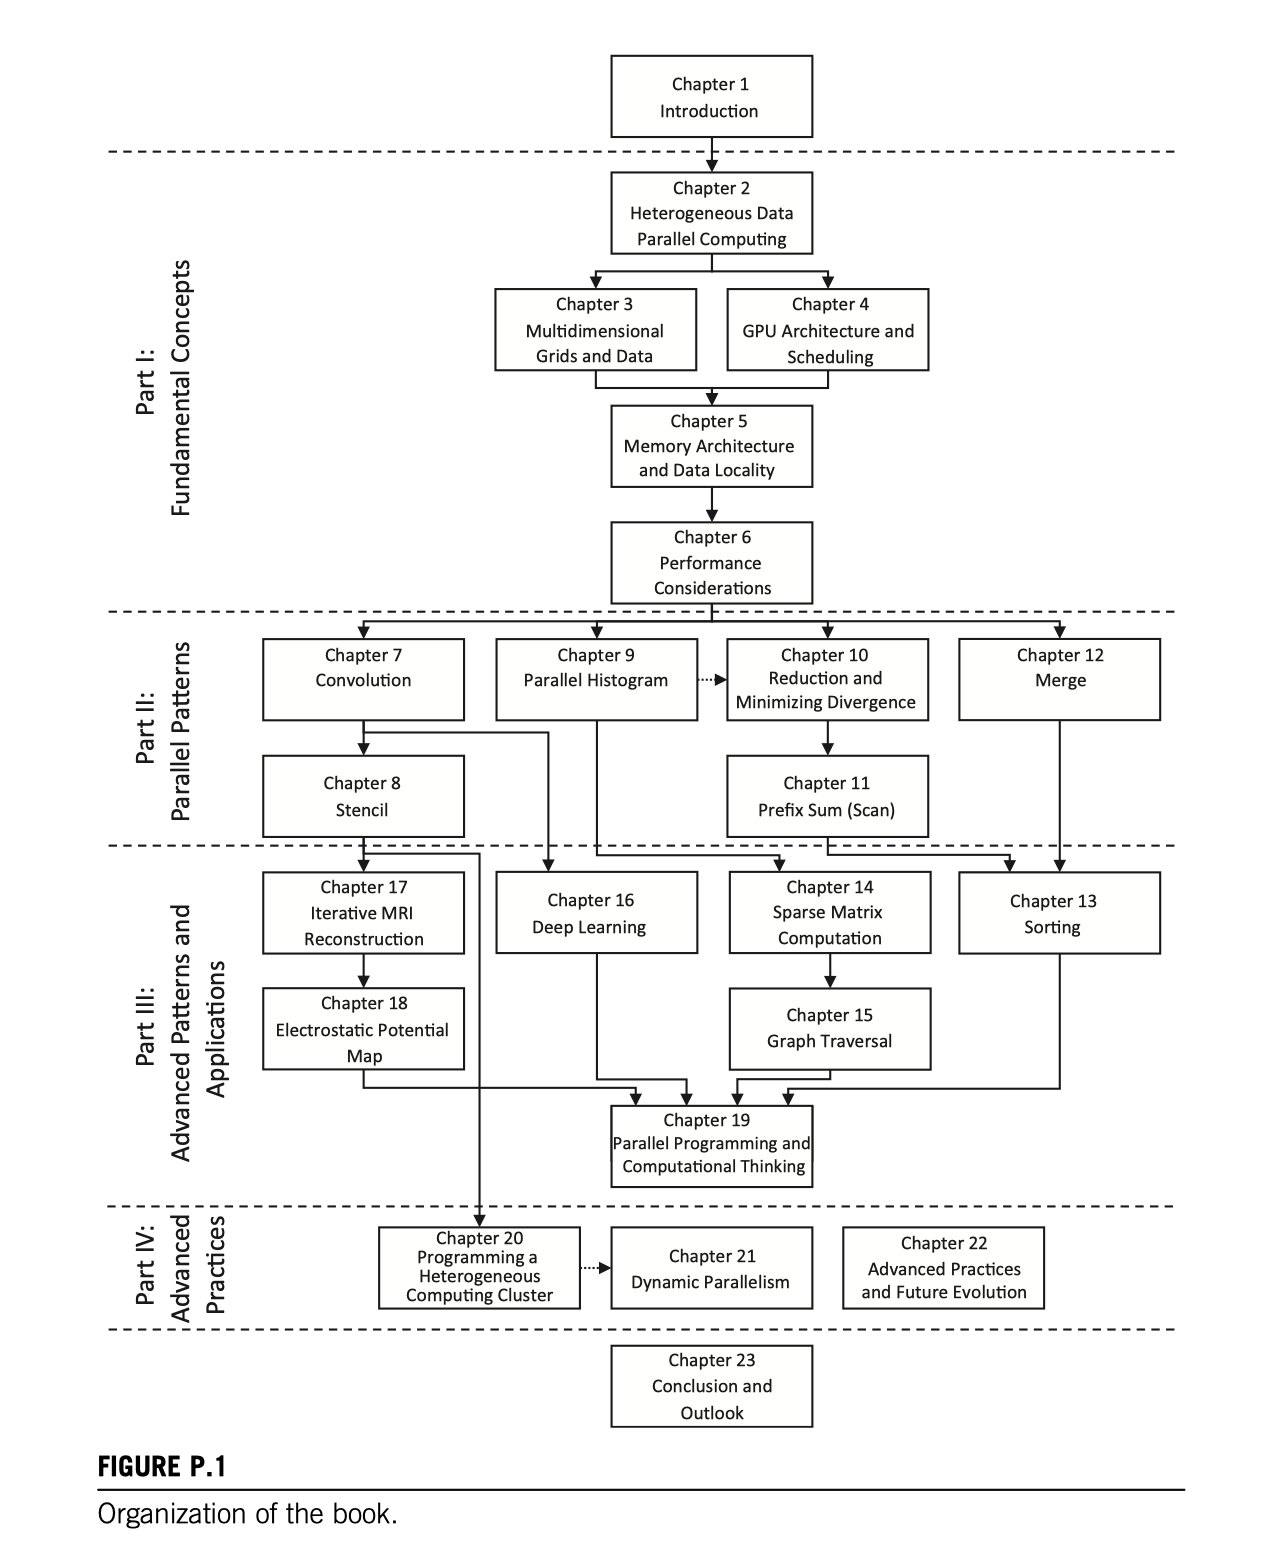
\includegraphics[width=\textwidth]{figs/P.1.png}
\end{figure}

\subsection{如何使用这本书}
我们希望通过本书提供一些教学课程的经验。 自 2006 年以来,我们教授多种类型的课程:一学期课程和一周强化课程。 
最初的 ECE498AL 课程已成为伊利诺伊大学香槟分校的永久课程,称为 ECE408 或 CS483。 
当我们第二次提供 ECE498AL 时,我们开始编写本书的一些早期章节。 
前四章也在 Nicolas Pinto 于 2009 年春天教授的麻省理工学院课程中进行了测试。
从那时起,我们将这本书用于 ECE408 的众多课程以及 Coursera 异构并行编程课程以及 VSCSE 和 PUMPS 暑期学校 。

\subsection{两阶段方法}
书中的大部分章节都设计为每节大约 75 分钟的讲座。 可能需要两节 75 分钟的讲座才能完全讲完的章节
是第 11 章(前缀和(扫描))、第 14 章(稀疏矩阵计算)和第 15 章(图遍历)。 
在 ECE408 中,讲座、编程作业和期末项目是同步进行的,并分为两个阶段。

在第一阶段,即本书的第一部分和第二部分,学生学习基础知识和基本模式,并练习通过指导性编程作业所学到的技能。 
此阶段由 12 章组成,通常需要大约 7 周的时间。 每周,学生都会完成与该周讲座相对应的编程作业。 
例如,第一周,基于第2章的讲座专门讲授基本的CUDA内存/线程模型、CUDA对C语言的扩展以及基本的编程工具。 
讲座结束后,学生可以在几个小时内编写简单的向量加法代码。

接下来的两周包括基于第 3 章到第 6 章的一系列四堂讲座,让学生对 CUDA 内存模型、CUDA 线程执行模型、
GPU 硬件性能特征和现代计算机系统架构有概念性的理解。 
在这两周内,学生们研究矩阵-矩阵乘法的不同实现,他们会看到在此期间其实现的性能如何显着提高。 
在剩下的四个星期中,讲座涵盖了基于第 7 章到第 12 章开发高性能并行应用程序所需的常见数据并行编程模式。
在这几周中,学生完成有关卷积、直方图、约简和前缀和的作业。 在第一阶段结束时,学生应该对并行编程非常熟悉,
并且应该准备好以更少的操作来实现更高级的代码。

在第二阶段(由第三部分和第四部分组成)中,学生在完成涉及加速高级模式或应用程序的最终项目时学习高级模式和应用程序。 
他们还学习了在完成项目时可能会发现有用的高级实践。 尽管我们通常不会在此阶段分配每周的编程作业,
但该项目通常有一个每周里程碑来帮助学生调整自己的节奏。 根据课程的持续时间和形式,教师可能无法涵盖此阶段的所有章节,
可能需要跳过一些章节。 教师还可以选择用客座讲座、论文讨论会或支持最终项目的讲座来代替一些讲座。 
因此,图 P.1 使用箭头来指示章节之间的依赖关系,以帮助教师选择可以跳过或重新排序的章节,以根据其特定上下文定制课程。

\subsection{将它们结合在一起:最终项目}
虽然本书的讲座、实验和章节有助于为学生奠定知识基础,但将学习经验整合在一起的是最终项目。 
最终项目对于整个学期的课程非常重要,因此它在课程中占据显着位置,需要近两个月的时间来重点关注。 
它包含五个创新方面:指导、研讨会、临床、最终报告和研讨会。 
虽然有关最终项目的大部分信息都可以在伊利诺伊州 NVIDIA GPU 教学套件中找到,但我们仍想提供这些方面设计背后的推理。

鼓励学生将他们的最终项目基于代表研究界当前挑战的问题。 为了推动这一过程,
教师应该招募几个计算科学研究小组来提出问题并担任导师。 导师被要求提供一份一到两页的项目规格表,
简要描述申请的重要性、导师希望与学生团队一起完成申请的目标、技术技能(特定类型的数学、物理) 和化学课程),
这是理解和使用应用程序所需的,以及学生可以利用的网络和传统资源列表,以获取技术背景、一般信息和构建块,
以及特定实现的特定 URL 或 FTP 路径 和编码示例。 
这些项目规格表还为学生提供了在其职业生涯后期定义自己的研究项目的学习经验。 
伊利诺伊州-NVIDIA GPU 教学套件中提供了几个示例。

\subsection{设计文档}
一旦学生决定了一个项目并组建了一个团队,他们就需要提交该项目的设计文件。 
这有助于他们在投入项目之前仔细考虑项目步骤。 进行此类规划的能力对于他们以后的职业成功非常重要。 
设计文件应讨论项目的背景和动机、应用程序级目标和潜在影响、最终应用程序的主要特征、
设计概述、实施计划、性能目标、验证计划和验收测试 ,以及项目进度表。

\subsection{项目报告及座谈会}
学生需要提交一份关于其团队主要发现的项目报告。 我们还建议举办全天的班级研讨会。 
在研讨会期间,学生使用与团队规模成比例的演示时段。 
在演示过程中,学生们为了全班同学的利益而突出了他们的项目报告中最好的部分。 
演讲占学生成绩的很大一部分。 每个学生必须单独回答针对该学生的问题,因此可以为同一团队中的个人分配不同的成绩。 
研讨会为学生提供了一个学习如何进行简洁演示的机会,以激励他们的同伴阅读全文。

\subsection{班级竞赛}
2016年ECE408的招生规模远远超过了最终项目进程所能容纳的水平。 结果,我们从期末项目变成了班级竞赛。 
在学期中期,我们宣布了一个竞赛挑战问题。 我们用一个讲座来解释比赛挑战问题以及用于对团队进行排名的规则。 
所有学生提交的内容都会自动评分和排名。 每个团队的最终排名取决于其并行代码的执行时间、正确性和清晰度。 
学生在学期结束时演示他们的解决方案并提交最终报告。 当班级规模导致最终项目不可行时,这种妥协保留了最终项目的一些好处。

\subsection{课程资源}
伊利诺伊州-NVIDIA GPU 教学套件是一个公开资源,其中包含讲座幻灯片和录音、实验作业、
最终项目指南以及为在课堂上使用本书的教师提供的示例项目规范。 此外,我们正在公开基于本书的伊利诺伊州本科生和研究生课程。 
虽然本书为这些课程提供了知识内容,但附加材料对于实现总体教育目标至关重要。

最后,我们鼓励您提交反馈。 如果您有任何改进本书的想法,我们希望收到您的来信。 我们想知道如何改进在线补充材料。 
当然,我们也想知道您喜欢这本书的哪些方面。 我们期待您的回音。


\newpage
\section*{致谢}
有很多人为第四版做出了特殊贡献。 我们首先要感谢各章节的合著者。 他们的名字列在他们做出特殊贡献的章节中。 
他们的专业知识对这个新版本的技术内容产生了巨大的影响。 如果没有这些人的专业知识和贡献,
我们就无法以我们希望向读者提供的洞察力来涵盖这些主题。

我们要特别感谢 CUDA 之父 Ian Buck 和 Tesla GPU 计算架构的首席架构师 John Nickolls。 
他们的团队为本课程构建了出色的基础设施。 NVIDIA 的许多工程师和研究人员也为 CUDA 的快速发展做出了贡献,
CUDA 支持高级并行模式的高效实现。 当我们制作第二版时,约翰去世了。 我们非常想念他。

自第三版以来,我们的外部审稿人花费了大量宝贵的时间为我们提供富有洞察力的反馈:
Sonia Lopez Alarcon(罗彻斯特理工学院)、Bedrich Benes(普渡大学)、Bryan Chin(加州大学圣地亚哥分校)、
Samuel Cho(维克森林大学) )、Kevin Farrell(爱尔兰都柏林布兰查兹敦理工学院)、
Lahouari Ghouti(沙特阿拉伯法赫德国王石油矿产大学)、Marisa Gil(西班牙巴塞罗那加泰罗尼亚理工大学)、
Karen L. Karavanic(波特兰) 州立大学)、Steve Lumetta(伊利诺伊大学厄巴纳-香槟分校)、
Dejan Milojici(惠普实验室)、Pinar Muyan-Ozcelik(加州州立大学萨克拉门托分校)、
Greg Peterson(田纳西大学诺克斯维尔分校)、Jose´L. Sa´nchez(卡斯蒂利亚拉曼恰大学)、
Janche Sang(克利夫兰州立大学)和 Jan Verschelde(伊利诺伊大学芝加哥分校)。 
他们的评论帮助我们显着提高了本书的内容和可读性。

Steve Merken、Kiruthika Govindaraju、Naomi Robertson 以及他们在爱思唯尔的员工为这个项目孜孜不倦地工作。

我们要特别感谢黄仁勋为开发这门课程提供了大量的财力和人力资源,为本书奠定了基础。

我们要感谢迪克·布拉胡特 (Dick Blahut),他向我们提出了启动该项目的挑战。 
Beth Katsinas 安排了 Dick Blahut 与 NVIDIA 副总裁 Dan Vivoli 的会面。 
通过那次聚会,Blahut 被介绍给 David,并挑战 David 来伊利诺伊州,与 Wen-mei. 一起创建原创的 ECE498AL 课程。

我们要特别感谢我们的同事 Kurt Akeley、Al Aho、Arvind、Dick Blahut、Randy Bryant、Bob Colwell、Bill Dally、
Ed Davidson、Mike Flynn、Michael Garland、John Hennessy、Pat Hanrahan、Nick Holonyak、Dick Karp、
Kurt Keutzer、Chris Lamb、Dave Liu、David Luebke、Dave Kuck、Nacho Navarro、Sanjay Patel、Yale Patt、
David Patterson、Bob Rao、Burton Smith、Jim Smith 和 Mateo Valero 花时间与我们分享了他们的见解 这些年来。

所有为这门课程和本书做出贡献的伟大人士的慷慨和热情让我们深感谦卑。


\newpage
\section{介绍}

自从计算出现以来,许多高价值应用程序都需要比计算设备所能提供的更高的执行速度和资源。 
早期应用依靠处理器速度、内存速度和内存容量的进步来增强应用级能力,如天气预报的及时性、工程结构分析的准确性、
计算机生成图形的真实性、航班预订数量等 每秒处理的资金转账数量。 
最近,深度学习等新应用程序需要比最好的计算设备所能提供的更多的执行速度和资源。 
这些应用需求在过去五年中推动了计算设备功能的快速进步,并且在可预见的未来将继续如此。

基于单个中央处理单元 (CPU) 的微处理器似乎按顺序步骤执行指令,例如 Intel 和 AMD 的 x86 处理器中的微处理器,
配备快速增加的时钟频率和硬件资源,推动了20世纪80年代和90年代的计算机应用性能的快速提高和成本的降低。 
在二十年的发展过程中,这些单 CPU 微处理器为桌面带来了 GFLOPS,即每秒千兆 ($10^9$) 次浮点运算,为数据中心带来了 TFLOPS,
即每秒万亿 ($10^{12}$) 次浮点运算。 这种对性能改进的不懈追求使得应用软件能够提供更多功能、
拥有更好的用户界面并生成更有用的结果。 反过来,一旦用户习惯了这些改进,他们就会要求更多的改进,
从而为计算机行业创造一个积极(良性)的循环。

然而,自 2003 年以来,由于能源消耗和散热问题,这种正向驱动的速度已经放缓。 
这些问题限制了时钟频率的增加以及单个 CPU 内每个时钟周期内可以执行的生产活动,同时保持了按顺序步骤执行指令的外观。 
从那时起,几乎所有微处理器供应商都转向了在每个芯片中使用多个物理 CPU(称为处理器内核)的模型,以提高处理能力。 
在这个模型中,传统的CPU可以被视为单核CPU。 为了受益于多个处理器内核,用户必须拥有多个指令序列,
无论是来自相同应用程序还是不同应用程序,都可以在这些处理器内核上同时执行。 对于要从多个处理器核心中受益的特定应用程序,
其工作必须分为可以在这些处理器核心上同时执行的多个指令序列。 
从单 CPU 按顺序执行指令到多核并行执行多个指令序列的转变对软件开发人员社区产生了巨大影响。

传统上,绝大多数软件应用程序都是作为顺序程序编写的,由处理器执行,
这些处理器的设计是冯·诺依曼在 1945 年的开创性报告中设想的(冯·诺依曼等人,1972 年)。 
人们可以将这些程序的执行理解为基于程序计数器(在文献中也称为指令指针)的概念按顺序单步执行代码。 
程序计数器包含处理器将执行的下一条指令的内存地址。 由应用程序的这种顺序、
逐步执行产生的指令执行活动序列在文献中被称为执行线程,或简称为线程。 线程的概念非常重要,
因此本书的其余部分将对其进行更正式的定义和广泛的使用。

从历史上看,大多数软件开发人员依赖硬件的进步,例如提高时钟速度和在后台执行多条指令,来提高顺序应用程序的速度; 
随着每一代新处理器的推出,相同的软件运行得更快。 计算机用户也越来越期望这些程序在每一代新一代微处理器上运行得更快。 
这种期望十多年来一直不成立。 顺序程序将仅在一个处理器内核上运行,一代又一代不会变得明显更快。 
如果没有性能改进,随着新微处理器的推出,应用程序开发人员将无法再在其软件中引入新的特性和功能; 
这减少了整个计算机行业的增长机会。

相反,每一代新一代微处理器将继续享受显着性能改进的应用软件将是并行程序,其中多个执行线程协作以更快地完成工作。 
并行程序相对于顺序程序的这种新的、显着提升的优势被称为并发革命(Sutter 和 Larus,2005)。 
并行编程的实践绝不是新鲜事。 几十年来,高性能计算 (HPC) 社区一直在开发并行程序。 
这些并行程序通常在昂贵的大型计算机上运行。 只有少数精英应用程序可以证明使用这些计算机是合理的,
从而将并行编程的实践限制在少数应用程序开发人员中。 现在所有新的微处理器都是并行计算机,
需要开发为并行程序的应用程序数量急剧增加。 现在软件开发人员非常需要学习并行编程,这也是本书的重点。

\subsection{异构并行计算}
自 2003 年以来,半导体行业已经确定了微处理器设计的两条主要轨迹(Hwu 等人,2008 年)。 
多核轨迹旨在在进入多核的同时保持顺序程序的执行速度。 多核始于两核处理器,并且核心数量随着每一代半导体工艺的发展而增加。 
最近的一个例子是最新的 Intel 多核服务器微处理器,具有多达 24 个处理器核心,每个处理器核心都是无序、多指令发布处理器,
实现完整的 x86 指令集,支持具有两个硬件线程的超线程,旨在最大限度地提高性能。 顺序程序的执行速度。 
另一个例子是最新的 ARM Ampere 多核服务器处理器,具有 128 个处理器内核。

相比之下,多线程轨迹更关注并行应用程序的执行吞吐量。 多线程轨迹始于大量线程,并且线程数量再次随着每一代的增加而增加。 
最近的一个例子是 NVIDIA Tesla A100 图形处理单元 (GPU),它具有数万个线程,在大量简单、有序的管道中执行。 
自 2003 年以来,多线程处理器,尤其是 GPU,一直在浮点性能竞赛中处于领先地位。
截至 2021 年,A100 GPU 的峰值浮点吞吐量为 64 位双精度 9.7 TFLOPS,32 位单精度 156 TFLOPS,
16 位半精度为 312 TFLOPS。 相比之下,最新的英特尔 24 核处理器的双精度峰值浮点吞吐量为 0.33 TLOPS,
单精度为 0.66 TFLOPS。 过去几年,多线程 GPU 和多核 CPU 之间的峰值浮点计算吞吐量之比一直在增加。 
这些不一定是应用程序速度; 它们只是这些芯片中执行资源可以支持的原始速度。

多核和多线程之间的峰值性能之间如此巨大的差距已经形成了显着的“电势”积累,在某些时候,必须做出一些让步。 
我们已经达到了这一点。 迄今为止,这种巨大的峰值性能差距已经促使许多应用程序开发人员将其软件的计算密集型部分转移到 
GPU 上执行。 也许更重要的是,并行执行性能的大幅提升使得革命性的新应用成为可能,例如本质上由计算密集型部分组成的深度学习。 
毫不奇怪,这些计算密集型部分也是并行编程的主要目标:当有更多工作要做时,
就有更多机会在协作的并行工作线程(即线程)之间分配工作。

{\color{red} Fig 1.1}

有人可能会问,为什么多线程 GPU 和多核 CPU 之间的峰值性能差距如此之大。 答案在于两种类型处理器之间基本设计理念的差异,
如图 1.1 所示。 如图 1.1A 所示,CPU 的设计针对顺序代码性能进行了优化。 
算术单元和操作数数据传送逻辑的设计旨在最大限度地减少算术运算的有效延迟,但代价是增加芯片面积和每单元功耗的使用。 
大型末级片上高速缓存旨在捕获频繁访问的数据,并将一些长延迟内存访问转换为短延迟高速缓存访问。 
复杂的分支预测逻辑和执行控制逻辑用于减轻条件分支指令的延迟。 通过减少操作的延迟,CPU 硬件减少了每个单独线程的执行延迟。 
然而,低延迟算术单元、复杂的操作数传送逻辑、大型高速缓冲存储器和控制逻辑消耗了芯片面积和功率,
否则这些芯片面积和功率可用于提供更多算术执行单元和存储器访问通道。 这种设计方法通常称为面向延迟的设计。

另一方面,GPU 的设计理念是由快速发展的视频游戏行业塑造的,
该行业对在高级游戏中执行大量浮点计算和每帧内存访问的能力提出了巨大的经济压力。 
这种需求促使 GPU 供应商寻找方法来最大化专用于浮点计算和内存访问吞吐量的芯片面积和功率预算。

在图形应用程序中,每秒执行大量浮点计算以完成视点变换和对象渲染等任务是非常直观的。 
此外,每秒执行大量内存访问的需求同样重要,甚至可能更重要。 
许多图形应用程序的速度受到数据从内存系统传送到处理器的速率的限制,反之亦然。 
GPU 必须能够将大量数据移入和移出其 DRAM(动态随机存取存储器)中的图形帧缓冲区,
因为这种移动可以使视频显示丰富并满足游戏玩家的需求。 
游戏应用程序普遍接受的宽松内存模型(各种系统软件、应用程序和 I/O 设备期望其内存访问工作的方式)
也使 GPU 更容易支持访问内存的大规模并行性。

相比之下,通用处理器必须满足传统操作系统、应用程序和 I/O 设备的要求,这些要求对支持并行内存访问提出了更多挑战,
从而使提高内存访问(通常称为内存)的吞吐量,常被称为内存带宽,变得更加困难。 
因此,图形芯片的运行内存带宽大约是同时可用 CPU 芯片的 10 倍,我们预计 GPU 在内存带宽方面将在一段时间内继续保持优势。

一个重要的观察是,就功耗和芯片面积而言,减少延迟比增加吞吐量要昂贵得多。 
例如,可以通过将运算单元的数量加倍来使运算吞吐量加倍,但代价是芯片面积和功耗加倍。 
然而,将算术延迟减少一半可能需要将电流加倍,但代价是所用芯片面积增加一倍以上,功耗增加四倍。 
因此,GPU 的主流解决方案是优化大量线程的执行吞吐量,而不是减少单个线程的延迟。 
这种设计方法允许流水线内存通道和算术运算具有较长的延迟,从而节省了芯片面积和功耗。 
内存访问硬件和算术单元的面积和功率的减少使得 GPU 设计者可以在芯片上拥有更多的硬件和算术单元,从而提高总执行吞吐量。 
图 1.1 通过在图 1.1A 的 CPU 设计中显示较少数量的较大算术单元和较少数量的内存通道,直观地说明了设计方法的差异,
与图 1.1B 中大量的较小算术单元和大量的存储器通道形成对比。

这些 GPU 的应用软件预计将使用大量并行线程编写。 当其中一些线程等待长延迟内存访问或算术运算时,
硬件会利用大量线程来寻找要做的工作。 图 1.1B 中的小型高速缓冲存储器用于帮助控制这些应用程序的带宽需求,
以便访问相同内存数据的多个线程不需要全部访问 DRAM。 这种设计风格通常称为面向吞吐量的设计,
因为它力求最大化大量线程的总执行吞吐量,同时允许单个线程可能需要更长的执行时间。

应该清楚的是,GPU 被设计为并行的、面向吞吐量的计算引擎,它们在某些 CPU 设计为能很好执行的任务上表现不佳。 
对于只有一个或很少线程的程序,具有较低操作延迟的CPU可以获得比GPU高得多的性能。 
当程序有大量线程时,具有较高执行吞吐量的GPU可以获得比CPU高得多的性能。 
因此,我们应该预料到许多应用程序会同时使用 CPU 和 GPU,在 CPU 上执行顺序部分,在 GPU 上执行数值密集型部分。 
这就是 NVIDIA 于 2007 年推出的统一计算设备架构 (CUDA) 编程模型旨在支持应用程序的 CPU-GPU 联合执行的原因。

还需要注意的是,当应用程序开发人员选择运行其应用程序的处理器时,速度并不是唯一的决定因素。 其他几个因素可能更为重要。 
首先也是最重要的是,所选处理器必须在市场上占有很大的份额,称为处理器的安装基础。 原因很简单。 
大量的客户群最能证明软件开发成本的合理性。 在市场份额较小的处理器上运行的应用程序不会有大量的客户群。 
这一直是传统并行计算系统的一个主要问题,与通用微处理器相比,传统并行计算系统的市场份额可以忽略不计。 
只有少数由政府和大公司资助的精英应用程序在这些传统的并行计算系统上成功开发。 多线程 GPU 改变了这种情况。 
由于 GPU 在 PC 市场的受欢迎,其销量已达数亿。 几乎所有台式电脑和高端笔记本电脑都配备了 GPU。 
迄今为止,已使用超过 10 亿个支持 CUDA 的 GPU。 如此庞大的市场占有率使这些 GPU 对应用程序开发人员来说具有经济吸引力。

另一个重要的决定因素是实用的外形因素和易于访问性。 直到 2006 年,并行软件应用程序都在数据中心服务器或部门集群上运行。 
但这样的执行环境往往会限制这些应用程序的使用。 比如在医学影像这样的应用中,发表一篇基于64节点集群机的论文就可以了。 
但磁共振成像 (MRI) 机器的实际临床应用是基于 PC 和特殊硬件加速器的某种组合。 
原因很简单,GE 和西门子等制造商无法在临床环境中销售需要计算机服务器机架的 MRI,而这在学术部门环境中很常见。 
事实上,美国国立卫生研究院 (NIH) 在一段时间内拒绝资助并行编程项目; 他们认为并行软件的影响将是有限的,
因为基于集群的大型机器无法在临床环境中工作。 如今,许多公司都配备了 GPU 的 MRI 产品,
美国国立卫生研究院 (NIH) 也资助使用 GPU 计算的研究。

直到 2006 年,图形芯片都非常难以使用,因为程序员必须使用相当于图形 API(应用程序编程接口)功能来访问处理单元,
这意味着需要 OpenGL 或 Direct3D 技术来对这些芯片进行编程。 更简单地说,计算必须表示为以某种方式绘制像素的函数,
以便在这些早期的 GPU 上执行。 该技术称为 GPGPU,用于使用 GPU 进行通用编程。 即使使用更高级别的编程环境,
底层代码仍然需要适合用于绘制像素的 API。 这些 API 限制了人们实际上可以为早期 GPU 编写的应用程序类型。 
因此,GPGPU 并没有成为一种广泛的编程现象。 尽管如此,这项技术还是足够令人兴奋,激发了一些英勇的努力和出色的研究成果。

2007 年,随着 CUDA 的发布,一切都发生了变化(NVIDIA,2007)。 CUDA 并不单独代表软件变更; 
芯片中添加了额外的硬件。 NVIDIA实际上专门投入了硅片面积以方便并行编程。 在 G80 及其后续并行计算芯片中,
GPGPU 程序根本不再通过图形接口。 相反,硅芯片上的新通用并行编程接口可以满足 CUDA 程序的要求。 
通用编程接口极大地扩展了可以轻松为 GPU 开发的应用程序类型。 所有其他软件层也都重新设计,
以便程序员可以使用熟悉的 C/C++ 编程工具。

虽然 GPU 是异构并行计算中的一类重要计算设备,但还有其他重要类型的计算设备在异构计算系统中用作加速器。 
例如,现场可编程门阵列已被广泛用于加速网络应用。 本书中介绍的使用 GPU 作为学习工具的技术也适用于这些加速器的编程任务。

\subsection{为什么要提高速度或并行性?}
正如我们在 1.1 节中所述,大规模并行编程的主要动机是让应用程序在未来的硬件世代中享受持续的速度提升。 
正如我们将在并行模式、高级模式和应用程序(第二部分和第三部分,第 7 章到第 19 章)中讨论的那样,
当应用程序适合并行执行时,在 GPU 上良好的实现可以比在单个 CPU 内核上顺序执行获得 100 倍以上的加速。
如果应用程序包含我们所说的“数据并行性”,通常只需几个小时的工作即可实现 10x 的加速。

人们可能会问为什么应用程序将继续要求提高速度。 我们今天拥有的许多应用程序似乎运行得足够快。 
尽管当今世界有无数的计算应用程序,但未来许多令人兴奋的大众市场应用程序都是我们之前认为的超级计算应用程序或超级应用程序。 
例如,生物学研究界正在越来越多地进入分子水平。 显微镜可以说是分子生物学中最重要的仪器,过去依赖光学或电子仪器。 
然而,我们使用这些仪器进行的分子水平观察存在局限性。 通过结合计算模型来模拟具有传统仪器设置的边界条件的基础分子活动,
可以有效地解决这些限制。 通过模拟,我们可以测量更多的细节并测试更多的假设,这比仅使用传统仪器所能想象的要多。 
在可预见的未来,就可建模的生物系统的规模以及可在可容忍响应时间内模拟的反应时间长度而言,这些模拟将继续受益于计算速度的提高。 
这些增强将对科学和医学产生巨大影响。

对于视频和音频编码和操作等应用,请考虑与旧式 NTSC 电视相比,我们对数字高清 (HD) 电视的满意度。 
一旦我们在高清电视上体验到图像的细节水平,就很难再回到旧技术了。 但请考虑高清电视所需的所有处理。 
这是一个高度并行的过程,三维 (3D) 成像和可视化也是如此。 
未来,视图合成和低分辨率视频的高分辨率显示等新功能将需要电视具有更高的计算能力。 
在消费者层面,我们将开始看到越来越多的视频和图像处理应用程序,这些应用程序可以改善图片和视频的焦点、光照和其他关键方面。

更高的计算速度带来的好处之一是更好的用户界面。 智能手机用户现在可以享受到与大屏幕电视相媲美的高分辨率触摸屏的更自然的界面。 
毫无疑问,这些设备的未来版本将整合具有 3D 视角的传感器和显示器、
结合虚拟和物理空间信息以增强可用性的应用程序以及基于语音和计算机视觉的界面,从而需要更高的计算速度。

消费电子游戏领域也正在进行类似的发展。 过去,在游戏中驾驶汽车只是一组预先安排好的场景。 
如果你的车撞到了障碍物,你的车的路线不会改变; 只是游戏比分发生了变化。 您的车轮没有弯曲或损坏,即使您失去了一个车轮,
驾驶也不再困难。 随着计算速度的提高,游戏可以基于动态模拟而不是预先安排的场景。 
我们可以期待在未来体验到更多这样的现实效果。 事故会损坏你的车轮,你的在线驾驶体验将会更加真实。 
精确建模物理现象的能力已经激发了数字孪生的概念,其中物理对象在模拟空间中具有精确的模型,
从而可以以更低的成本彻底进行压力测试和恶化预测。 众所周知,物理效应的真实建模和模拟需要非常大量的计算能力。

通过大幅提高计算吞吐量而实现的新应用程序的一个重要例子是基于人工神经网络的深度学习。 
虽然神经网络自 20 世纪 70 年代以来一直在积极研究,但它们在实际应用中一直无效,
因为训练这些网络需要太多的标记数据和太多的计算。 互联网的兴起提供了大量带标签的图片,GPU 的兴起带来了计算吞吐量的激增。 
因此,自 2012 年以来,基于神经网络的应用在计算机视觉和自然语言处理领域得到了快速采用。
这种采用彻底改变了计算机视觉和自然语言处理应用,并引发了自动驾驶汽车和家庭辅助设备的快速发展。

我们提到的所有新应用程序都涉及以不同方式和在不同级别模拟和/或表示物理并发世界,并处理大量数据。 
有了如此大量的数据,大部分计算可以在数据的不同部分上并行完成,尽管它们必须在某些时候进行协调。 
在大多数情况下,数据交付的有效管理会对并行应用程序的可实现速度产生重大影响。 
虽然这样做的技术通常为一些每天使用此类应用程序的专家所熟知,
但绝大多数应用程序开发人员可以从对这些技术的更直观的理解和实际工作知识中受益。

我们的目标是以直观的方式向应用程序开发人员展示数据管理技术,这些开发人员的正规教育可能不是计算机科学或计算机工程。 
我们还旨在提供许多实用的代码示例和实践练习,帮助读者获取工作知识,
这需要一个实用的编程模型来促进并行实现并支持数据交付的正确管理。 CUDA 提供了这样的编程模型,
并且已经过大型开发者社区的充分测试。

\subsection{加速实际的应用}
通过并行化应用程序,我们可以期望获得多少加速? 计算系统 A 相对于计算系统 B 的应用程序加速比的定义是,
在系统 B 中执行应用程序所用的时间与在系统 A 中执行相同应用程序所用的时间之比。
例如,如果应用程序在系统 A 中执行需要花费 10 秒,而在系统 B 中执行需要 200 秒,
则系统 A 相对于系统 B 的执行加速为 200/10=20,称为 20x(20 倍)加速。

并行计算系统相对于串行计算系统可实现的加速取决于可以并行化的应用程序部分。 
例如,如果可并行部分所花费的时间百分比为 30\%,则并行部分加速 100x 将使应用程序的总执行时间减少不超过 29.7\%。 
也就是说,整个应用程序的加速大约仅为 1/(1 - 0.297)=1.42x。 事实上,即使在并行部分进行无限量的加速,
也只能将执行时间减少 30\%,实现的加速不超过 1.433。 
通过并行执行可以实现的加速水平可能会受到应用程序的可并行部分的严重限制,这一事实被称为阿姆达尔定律(Amdahl,2013)。 
另一方面,如果 99\% 的执行时间都在并行部分,则并行部分加速 100x 会将应用程序执行时间减少到原始时间的 1.99\%。 
这使整个应用程序加速了 50x。 因此,对于大规模并行处理器来说,应用程序的绝大多数执行都在并行部分进行,
以有效加快其执行速度,这一点非常重要。

研究人员已在某些应用程序中实现了超过 100x 的加速。 然而,这通常只有在算法得到增强后进行大量优化和调整才能实现,
这样超过 99.9\% 的应用程序工作都在并行部分。

应用程序可实现的加速水平的另一个重要因素是从内存访问和写入数据的速度。 在实践中,
应用程序的直接并行化通常会导致内存 (DRAM) 带宽饱和,从而仅带来大约 10x 的加速。 诀窍在于找出如何解决内存带宽限制,
这涉及到进行多种转换之一,以利用专门的 GPU 片上内存来大幅减少对 DRAM 的访问次数。 
然而,必须进一步优化代码以克服片上内存容量有限等限制。 本书的一个重要目标是帮助读者充分理解这些优化并熟练使用它们。

请记住,单核 CPU 执行所实现的加速水平也可以反映 CPU 对应用程序的适用性。 在某些应用程序中,CPU 的性能非常好,
这使得使用 GPU 加速性能变得更加困难。 大多数应用程序都有一些可以由 CPU 更好地执行的部分。 
我们必须给CPU一个公平的执行机会,并确保编写的代码能够让GPU补充CPU的执行,
从而正确地利用CPU/GPU组合系统的异构并行计算能力。 
截至目前,结合了多核 CPU 和众核 GPU 的大众市场计算系统已经为笔记本电脑带来了万亿级计算,为集群带来了百亿亿级计算。

{\color{red} Fig 1.2}

图 1.2 说明了典型应用的主要部分。 实际应用程序的大部分代码往往是连续的。 这些连续的部分被图示为桃子的“核”区域; 
尝试将并行计算技术应用于这些部分就像咬桃核一样——感觉不太好! 这些部分很难并行化。 CPU 在这些部分往往做得非常好。 
好消息是,虽然这些部分可能占用大部分代码,但它们往往只占超级应用程序执行时间的一小部分。

然后是我们所说的“桃肉”部分。 这些部分很容易并行化,一些早期的图形应用程序也是如此。 
异构计算系统中的并行编程可以极大地提高这些应用程序的速度。 如图1.2所示,早期的GPGPU编程接口只覆盖了桃肉部分的一小部分,
这类似于最令人兴奋的应用程序的一小部分。 正如我们将看到的,CUDA 编程接口旨在涵盖令人兴奋的应用程序的更大部分。 
并行编程模型及其底层硬件仍在快速发展,以实现更大的应用程序部分的高效并行化。

\subsection{并行编程中的挑战}
是什么让并行编程变得困难? 有人曾经说过,如果不关心性能,并行编程是很容易的。 您实际上可以在一小时内编写一个并行程序。 
但是,如果您不关心性能,为什么还要编写并行程序呢?

本书解决了在并行编程中实现高性能的几个挑战。 首先,设计具有与顺序算法相同的算法(计算)复杂度的并行算法可能具有挑战性。 
许多并行算法执行与顺序算法相同的工作量。 然而,一些并行算法比顺序算法做更多的工作。 事实上,有时他们可能会做太多的工作,
以至于最终在大型输入数据集上运行速度变慢。 这尤其是一个问题,因为快速处理大型输入数据集是并行编程的重要动机。

例如,许多现实世界的问题最自然地用数学递归来描述。 并行化这些问题通常需要以非直观的方式思考问题,
并且可能需要在执行过程中进行冗余工作。 有一些重要的算法原语,例如前缀和,可以促进将问题的顺序递归公式转换为更并行的形式。 
我们将更正式地介绍工作效率的概念,并将说明设计并行算法所涉及的方法和权衡,
这些算法可以使用重要的并行模式(例如第 11 章“前缀”中的前缀和)实现与顺序算法相同水平的计算复杂性 总和(扫描)。

其次,许多应用程序的执行速度受到内存访问延迟和/或吞吐量的限制。 我们将这些应用程序称为内存限制应用程序; 
相比之下,计算密集型应用程序受到每字节数据执行的指令数量的限制。 
在内存受限的应用程序中实现高性能并行执行通常需要提高内存访问速度的方法。 
我们将在第 5 章“内存架构和数据局部性”和第 6 章“性能注意事项”中介绍内存访问的优化技术,
并将在有关并行模式和应用程序的几个章节中应用这些技术。

第三,并行程序的执行速度通常比顺序程序的情况对输入数据特征更敏感。 许多现实世界的应用程序需要处理具有广泛变化特征的输入,
例如不稳定或不可预测的数据大小以及不均匀的数据分布。 这些大小和分布的变化可能会导致分配给并行线程的工作量不均匀,
并可能显着降低并行执行的效率。 并行程序的性能有时会因这些特征而发生巨大变化。 
我们将在介绍并行模式和应用程序的章节中介绍用于规范数据分布和/或动态细化线程数量的技术,以应对这些挑战。

第四,某些应用程序可以并行化,同时几乎不需要跨不同线程进行协作。 这些应用程序通常被称为“令人尴尬的并行”。 
其他应用程序需要线程相互协作,这需要使用同步操作,例如屏障或原子操作。 这些同步操作给应用程序带来了开销,
因为线程经常会发现自己在等待其他线程而不是执行有用的工作。 我们将在本书中讨论减少同步开销的各种策略。

幸运的是,研究人员已经解决了大部分挑战。 跨应用程序域还存在一些常见模式,
使我们能够将在一个域中派生的解决方案应用于其他域中的挑战。 
这是我们将在重要的并行计算模式和应用程序的背景下提出解决这些挑战的关键技术的主要原因。

\subsection{相关并行编程接口}
在过去的几十年里,人们提出了许多并行编程语言和模型(Mattson 等,2004)。 
最广泛使用的是用于共享内存多处理器系统的 OpenMP(Open,2005)和用于可扩展集群计算的消息传递接口(MPI)(MPI,2009)。 
两者都已成为主要计算机供应商支持的标准化编程接口。

OpenMP 实现由编译器和运行时组成。 程序员向 OpenMP 编译器指定有关循环的指令(命令)和编译指示(提示)。 
通过这些指令和编译指示,OpenMP 编译器可以生成并行代码。 运行时系统通过管理并行线程和资源来支持并行代码的执行。 
OpenMP 最初是为 CPU 执行而设计的,现已扩展为支持 GPU 执行。 OpenMP 的主要优点是它提供编译器自动化和运行时支持,
以从程序员那里抽象出许多并行编程细节。 
这种自动化和抽象有助于使应用程序代码在不同供应商生产的系统以及同一供应商的不同代系统之间更加可移植。 
我们将此属性称为性能可移植性。 然而,在 OpenMP 中进行有效的编程仍然需要程序员了解所涉及的所有详细的并行编程概念。 
由于 CUDA 为程序员提供了对这些并行编程细节的明确控制,因此即使对于那些想要使用 OpenMP 作为主要编程接口的人来说,
它也是一种极好的学习工具。 此外,根据我们的经验,OpenMP 编译器仍在不断发展和改进。 
许多程序员可能需要使用 CUDA 风格的接口来处理 OpenMP 编译器无法满足的部分。

另一方面,MPI 是一种编程接口,其中集群中的计算节点不共享内存(MPI,2009)。 
所有的数据共享和交互都必须通过显式的消息传递来完成。 MPI在HPC中得到了广泛的应用。 
用MPI编写的应用程序已在超过10万个节点的集群计算系统上成功运行。 如今,许多 HPC 集群都采用异构 CPU/GPU 节点。 
由于计算节点之间缺乏共享内存,将应用程序移植到 MPI 所需的工作量可能相当大。 
程序员需要执行域分解以跨各个节点划分输入和输出数据。 在域分解的基础上,
程序员还需要调用消息发送和接收函数来管理节点之间的数据交换。 相比之下,
CUDA 为 GPU 中的并行执行提供共享内存来解决这一难题。 虽然 CUDA 是与每个节点的有效接口,
但大多数应用程序开发人员需要使用 MPI 在集群级别进行编程。 
此外,通过 NVIDIA Collective Communications Library (NCCL) 等 API,CUDA 中的多 GPU 编程支持不断增加。 
因此,HPC 中的并行程序员了解如何在使用多 GPU 节点的现代计算集群中进行联合 MPI/CUDA 编程非常重要,
该主题将在第 20 章“异构计算集群编程”中介绍。

2009 年,包括 Apple、Intel、AMD/ATI 和 NVIDIA 在内的几家主要行业参与者联合开发了一种名为
开放计算语言 (OpenCL) 的标准化编程模型(The Khronos Group,2009)。 与 CUDA 类似,
OpenCL 编程模型定义了语言扩展和运行时 API,以允许程序员管理大规模并行处理器中的并行性和数据交付。 
与 CUDA 相比,OpenCL 更多地依赖 API,更少地依赖语言扩展。 
这使得供应商能够快速调整其现有的编译器和工具来处理 OpenCL 程序。 OpenCL 是一种标准化的编程模型,
用 OpenCL 开发的应用程序无需修改即可在所有支持 OpenCL 语言扩展和 API 的处理器上正确运行。 
然而,人们可能需要修改应用程序才能实现新处理器的高性能。

熟悉 OpenCL 和 CUDA 的人都知道,OpenCL 和 CUDA 的关键概念和功能之间存在显着的相似性。 
也就是说,CUDA程序员可以以最小的努力学习OpenCL编程。 更重要的是,
几乎所有在使用 CUDA 中学到的技术都可以轻松应用于 OpenCL 编程。

\subsection{总体目标}
我们的主要目标是教读者如何对大规模并行处理器进行编程以实现高性能。 
因此,本书的大部分内容都致力于开发高性能并行代码的技术。 我们的方法不需要大量的硬件专业知识。 
然而,您需要对并行硬件架构有一个很好的概念性理解,以便能够推断代码的性能行为。 
因此,我们将用一些篇幅来直观地理解基本的硬件架构特性,并用许多篇幅来介绍开发高性能并行程序的技术。 
特别是,我们将重点关注计算思维(Wing,2006)技术,这些技术将使您能够以适合大规模并行处理器上高性能执行的方式思考问题。

大多数处理器上的高性能并行编程需要了解硬件的工作原理。 可能需要很多年才能构建工具和机器,
使程序员能够在没有这些知识的情况下开发高性能代码。 即使我们有这样的工具,
我们怀疑了解硬件知识的程序员将能够比那些不了解硬件的程序员更有效地使用这些工具。 
因此,我们专门用第 4 章“计算架构和调度”来介绍 GPU 架构的基础知识。 
作为高性能并行编程技术讨论的一部分,我们还讨论了更专业的体系结构概念。

我们的第二个目标是教授并行编程的正确功能和可靠性,这是并行计算中的一个微妙问题。 
过去从事并行系统工作的程序员都知道,仅实现初始性能是不够的。 挑战在于以一种可以调试代码并支持用户的方式来实现它。 
CUDA 编程模型鼓励使用简单形式的屏障同步、内存一致性和原子性来管理并行性。 
此外,它还提供了一系列强大的工具,使人们不仅可以调试功能方面,还可以调试性能瓶颈。 
我们将证明,通过关注数据并行性,可以在应用程序中实现高性能和高可靠性。

我们的第三个目标是通过探索并行编程方法来实现未来硬件各代的可扩展性,
以便未来的机器(将越来越并行)可以比今天的机器更快地运行代码。 我们希望帮助您掌握并行编程,
以便您的程序可以扩展到新一代机器的性能水平。 这种可扩展性的关键是规范和本地化内存数据访问,
以最大限度地减少关键资源的消耗和更新数据结构时的冲突。 
因此,开发高性能并行代码的技术对于确保应用程序未来的可扩展性也很重要。

实现这些目标需要大量的技术知识,因此我们将在本书中介绍并行编程的相当多的原理和模式(Mattson et al., 2004)。 
我们不会单独教授这些原则和模式。 我们将在并行化有用应用程序的背景下教授他们。 
然而,我们无法涵盖所有这些技术,因此我们选择了最有用且经过充分验证的技术来详细介绍。 
事实上,当前版本有关并行模式的章节数量显着增加。 现在我们准备向您提供本书其余部分的快速概述。

\subsection{本书的组织}
本书分为四个部分。 第一部分涵盖并行编程、数据并行、GPU 和性能优化的基本概念。 
这些基础章节为读者提供了成为 GPU 程序员所需的基本知识和技能。 第二部分介绍了原始并行模式,
第三部分介绍了更高级的并行模式和应用程序。 这两部分应用了第一部分中学到的知识和技能,
并根据需要介绍了其他 GPU 架构特性和优化技术。 最后一部分(第四部分)介绍了高级实践,
以帮助想要成为专家 GPU 程序员的读者完善知识。

关于基本概念的第一部分由第 2 章至第 6 章组成。 第 2 章,异构数据并行计算,介绍数据并行性和 CUDA C 编程。 
本章依赖于读者之前具有 C 编程经验的事实。 它首先介绍了 CUDA C 作为 C 的简单、小型扩展,
支持异构 CPU/GPU 计算和广泛使用的单程序、多数据并行编程模型。 
然后,它涵盖了以下方面所涉及的思维过程:(1) 识别要并行化的应用程序部分,
(2) 隔离并行化代码要使用的数据,使用 API 函数在并行计算设备上分配内存, (3)使用API函数将数据传输到并行计算设备,
(4)将并行部分开发为将由并行线程执行的内核函数,(5)启动由并行线程执行的内核函数,
以及( 6) 最终通过 API 函数调用将数据传输回主机处理器。 我们使用向量加法的运行示例来说明这些概念。 
虽然本章的目标是教授 CUDA C 编程模型的足够概念,以便读者能够编写简单的并行 CUDA C 程序,
但它涵盖了开发基于任何并行编程接口的并行应用程序所需的几种基本技能。

第 3 章“多维网格和数据”介绍了 CUDA 并行执行模型的更多细节,特别是它涉及使用线程的多维组织处理多维数据。 
它对线程的创建、组织、资源绑定和数据绑定提供了足够的洞察力,使读者能够使用 CUDA C 实现复杂的计算。

第 4 章,计算架构和调度,介绍 GPU 架构,重点介绍如何组织计算核心以及如何调度线程在这些核心上执行。 
讨论了各种架构注意事项,以及它们对 GPU 架构上执行的代码性能的影响。 其中包括透明可扩展性、SIMD 执行和控制发散、
多线程和延迟容忍以及占用等概念,所有这些都在本章中进行了定义和讨论。

第 5 章“内存架构和数据局部性”通过讨论 GPU 的内存架构来扩展第 4 章“计算架构和调度”。 
它还讨论了可用于保存 CUDA 变量以管理数据传输和提高程序执行速度的特殊存储器。 
我们介绍分配和使用这些内存的 CUDA 语言功能。 适当地使用这些存储器可以极大地提高数据访问吞吐量,
并有助于缓解存储器系统中的流量拥塞。

第 6 章“性能注意事项”介绍了当前 CUDA 硬件中的几个重要的性能注意事项。 
特别是,它提供了有关所需的线程执行和内存访问模式的更多详细信息。 
这些细节构成了程序员推理其组织计算和数据决策的后果的概念基础。 
本章最后列出了 GPU 程序员经常用来优化任何计算模式的常见优化策略清单。 
该清单将在本书的接下来的两部分中使用,以优化各种并行模式和应用程序。

关于原始并行模式的第二部分由第 7 章至第 12 章组成。 第 7 章“卷积”介绍了卷积,这是一种常用的并行计算模式,
植根于数字信号处理和计算机视觉,需要仔细管理数据访问局部性。 我们还使用这种模式在现代 GPU 中引入恒定内存和缓存。 
第 8 章“模板”介绍了模板,这是一种类似于卷积的模式,但植根于求解微分方程,
并且具有为进一步优化数据访问局部性提供独特机会的特定功能。 我们还使用此模式来介绍线程和数据的 3D 组织,
并展示第 6 章“性能注意事项”中介绍的针对线程粒度的优化。

第 9 章“并行直方图”介绍了直方图,这是一种广泛用于统计数据分析以及大型数据集中的模式识别的模式。 
我们还使用这种模式引入原子操作作为协调共享数据并发更新和私有化优化的手段,从而减少了这些操作的开销。 
第 10 章“归约和最小化分支”介绍了归约树模式,该模式用于总结输入数据的集合。 
我们还使用此模式来演示控制分支发散对性能的影响,并展示如何减轻这种影响的技术。 
第 11 章“前缀和(扫描)”介绍了前缀和或扫描,这是一种重要的并行计算模式,它将固有的顺序计算转换为并行计算。 
我们还使用这种模式来引入并行算法中工作效率的概念。 最后,第 12 章“合并”介绍了并行合并,
这是一种在分而治之工作分区策略中广泛使用的模式。 我们还用本章来介绍动态输入数据的识别和组织。

关于高级并行模式和应用程序的第三部分在精神上与第二部分类似,但所涵盖的模式更详细,并且通常包含更多应用程序上下文。 
因此,这些章节不太关注介绍新技术或功能,而是更关注特定于应用程序的注意事项。 对于每个应用程序,
我们首先确定制定并行执行基本结构的替代方法,然后推理每个替代方案的优点和缺点。 
然后,我们完成实现高性能所需的代码转换步骤。 这些章节帮助读者将前面章节中的所有材料放在一起,
并在他们承担自己的应用程序开发项目时为他们提供支持。

第三部分由第 13 章至第 19 章组成。 第 13 章“排序”介绍了并行排序的两种形式:基数排序和合并排序。 
这种高级模式利用了前面章节中介绍的更原始的模式,特别是前缀和和并行合并。 第 14 章,稀疏矩阵计算,介绍了稀疏矩阵计算,
它广泛用于处理非常大的数据集。 本章向读者介绍了重新排列数据以实现更有效的并行访问的概念:数据压缩、填充、排序、转置
和正则化。 第 15 章,图遍历,介绍图算法以及如何在 GPU 编程中有效地实现图搜索。 提出了许多不同的并行图算法策略,
并讨论了图结构对最佳算法选择的影响。 这些策略建立在更原始的模式之上,例如直方图和合并。

第 16 章“深度学习”涵盖了深度学习,它正在成为 GPU 计算的一个极其重要的领域。 我们介绍了卷积神经网络的有效实现,
并将更深入的讨论留给其他来源。 卷积神经网络的高效实现利用了平铺等技术和卷积等模式。 第 17 章,迭代磁共振成像重建,
涵盖非笛卡尔 MRI 重建以及如何利用循环融合和分散-聚集变换等技术来增强并行性并减少同步开销。 第 18 章,静电势图,
涵盖了分子可视化和分析,这得益于通过应用稀疏矩阵计算中的经验教训来处理不规则数据的技术。

第 19 章“并行编程和计算思维”介绍了计算思维,即以更适合 HPC 的方式制定和解决计算问题的艺术。 
它通过涵盖组织程序的计算任务以使它们可以并行完成的概念来实现这一点。 我们首先讨论将抽象的科学、
特定问题的概念组织成计算任务的转化过程,这是生产高质量串行或并行应用软件的重要的第一步。 
然后本章讨论并行算法结构及其对应用程序性能的影响,这是基于 CUDA 性能调优经验。 
尽管我们没有深入探讨这些替代并行编程风格的实现细节,
但我们希望读者能够利用在本书中获得的基础来学习其中任何一种编程风格的编程。 
我们还提出了一个高级案例研究,以展示通过创造性计算思维可以看到的机会。

第四部分高级实践由第 20 至 22 章组成。 第 20 章,异构计算集群编程,介绍了异构集群上的 CUDA 编程,
其中每个计算节点都由 CPU 和 GPU 组成。 
我们讨论使用 MPI 和 CUDA 来集成节点间计算和节点内计算以及由此产生的通信问题和实践。 
第 21 章“CUDA 动态并行性”介绍了动态并行性,即 GPU 根据数据或程序结构动态为自身创建工作的能力,
而不是总是等待 CPU 这样做。 第 22 章“高级实践和未来发展”列出了 CUDA 程序员需要了解的重要的各种高级功能和实践。 
其中包括零复制内存、统一虚拟内存、多个内核同时执行、函数调用、异常处理、调试、分析、双精度支持、
可配置缓存/暂存器大小等主题。 例如,早期版本的 CUDA 在 CPU 和 GPU 之间提供有限的共享内存功能。 
程序员需要显式管理 CPU 和 GPU 之间的数据传输。 然而,当前版本的 CUDA 支持统一虚拟内存和零拷贝内存等功能,
可实现 CPU 和 GPU 之间的数据无缝共享。 有了这样的支持,CUDA 程序员可以将变量和数据结构声明为在 CPU 和 GPU 之间共享。 
运行时硬件和软件保持一致性,并根据需要自动代表程序员执行优化的数据传输操作。 
这种支持显着降低了与计算和 I/O 活动重叠的数据传输所涉及的编程复杂性。 在教科书的介绍部分,
我们使用 API 进行显式数据传输,以便读者更好地了解幕后发生的情况。 
我们稍后会在第 22 章“高级实践和未来演进”中介绍统一虚拟内存和零拷贝内存。

虽然本书中的章节都是基于 CUDA 的,但它们总体上帮助读者建立了并行编程的基础。 
我们相信,当我们从具体的例子中学习时,人类能够最好地理解。 也就是说,我们必须首先在特定编程模型的上下文中学习概念,
这为我们将知识推广到其他编程模型时提供了坚实的基础。 当我们这样做时,我们可以从 CUDA 示例中汲取具体经验。 
对CUDA的深入体验也使我们变得成熟,这将有助于我们学习甚至可能与CUDA模型无关的概念。

第 23 章“结论和展望”提供了结论性意见以及对大规模并行编程的未来的展望。 我们首先重新审视我们的目标,
并总结各章如何组合在一起以帮助实现目标。 最后,我们预测大规模并行计算的快速进步将使其成为未来十年最令人兴奋的领域之一。


\newpage
\section{异构数据并行计算}

数据并行是指对数据集的不同部分执行的计算工作可以彼此独立地完成,从而可以彼此并行地完成的现象。 许多应用程序表现出丰富的数据并行性,这使得它们适合可扩展的并行执行。 因此,并行程序员熟悉数据并行性的概念以及编写利用数据并行性的代码的并行编程语言结构非常重要。 在本章中,我们将使用 CUDA C 语言结构来开发一个简单的数据并行程序。

\subsection{数据并行}
当现代软件应用程序运行缓慢时,问题通常是数据——数据太多而无法处理。 图像处理应用程序处理具有数百万到数万亿像素的图像或视频。 科学应用程序使用数十亿个网格点对流体动力学进行建模。 分子动力学应用必须模拟数千到数十亿个原子之间的相互作用。 航空公司的调度涉及数千个航班、机组人员和机场登机口。 大多数像素、粒子、网格点、交互、飞行等通常可以在很大程度上独立处理。 例如,在图像处理中,将彩色像素转换为灰度仅需要该像素的数据。 模糊图像会平均每个像素的颜色与附近像素的颜色,仅需要该小像素邻域的数据。 即使是看似全局的操作,例如查找图像中所有像素的平均亮度,也可以分解为许多可以独立执行的较小计算。 这种对不同数据块的独立评估是数据并行性的基础。 编写数据并行代码需要(重新)组织围绕数据的计算,以便我们可以并行执行最终的独立计算,从而更快地完成整个工作——通常要快得多。

让我们通过一个彩色到灰度转换的例子来说明数据并行的概念。 图 2.1 显示了由许多像素组成的彩色图像(左侧),每个像素包含从 0(黑色)到 1(全强度)变化的红色、绿色和蓝色分数值(r、g、b)。

为了将彩色图像(图 2.1 左侧)转换为灰度图像(右侧),我们通过应用以下加权和公式计算每个像素的亮度值 L:
\begin{equation*}
	L = r*0.21 + g*0.72 + b * 0.07
\end{equation*}

\begin{remark}[RGB 彩色图像表示]
	在 RGB 表示中,图像中的每个像素都存储为 (r, g, b) 值的元组。 图像行的格式为 (r g b) (r g b) 。 。 。 (r g b),如下面的概念图所示。 每个元组指定红色 (R)、绿色 (G) 和蓝色 (B) 的混合。 也就是说,对于每个像素,r、g、b 值代表渲染该像素时红、绿、蓝光源的强度(0 为暗,1 为全强度)。

这三种颜色的实际允许混合因行业指定的颜色空间而异。 这里,AdbobeRGBt 颜色空间中三种颜色的有效组合显示为三角形的内部。 每个混合的垂直坐标(y 值)和水平坐标(x 值)显示应为 G 和 R 的像素强度分数。像素强度的剩余分数 (1-yÀx) 应分配给 B。 渲染图像时,每个像素的 r、g、b 值用于计算像素的总强度(亮度)以及混合系数(x、y、1-y-x)。
\end{remark}

如果我们将输入视为由 RGB 值数组 I 组织的图像,并将输出视为相应的亮度值数组 O,则我们得到如图 2.2 所示的简单计算结构。 例如,根据上式计算I[0]中RGB值的加权和,生成O[0]; O[1]是通过计算I[1]中RGB值的加权和生成的; O[2]是通过计算I[2]中RGB值的加权和生成的; 等等。 这些每像素计算都不相互依赖。 所有这些都可以独立执行。 显然,彩色到灰度的转换表现出丰富的数据并行性。 当然,完整应用程序中的数据并行性可能更加复杂,本书的大部分内容都致力于教授发现和利用数据并行性所必需的并行思维。

\begin{remark}[任务并行与数据并行]
数据并行并不是并行编程中使用的唯一并行类型。 任务并行性也广泛应用于并行编程中。 任务并行性通常通过应用程序的任务分解来暴露。 例如,一个简单的应用程序可能需要进行向量加法和矩阵向量乘法。 其中每一个都是一项任务。 如果两个任务可以独立完成,则存在任务并行性。 I/O 和数据传输也是常见的任务源。

在大型应用程序中,通常存在大量独立任务,因此任务并行性也较大。 例如,在分子动力学模拟器中,自然任务列表包括振动力、旋转力、非键合力的邻居识别、非键合力、速度和位置以及基于速度和位置的其他物理属性。

一般来说,数据并行性是并行程序可扩展性的主要来源。 对于大型数据集,人们通常可以找到丰富的数据并行性,以便能够利用大规模并行处理器,并允许应用程序性能随着每一代具有更多执行资源的硬件而增长。 尽管如此,任务并行性也可以在实现性能目标方面发挥重要作用。 稍后在介绍流时我们将介绍任务并行性。
\end{remark}

\subsection{CUDA C程序结构}
我们现在准备学习如何编写 CUDA C 程序来利用数据并行性来加快执行速度。 CUDA C 1 以最少的新语法和库函数扩展了流行的 ANSI C 编程语言,使程序员能够针对包含 CPU 内核和大规模并行 GPU 的异构计算系统。 顾名思义,CUDA C 构建在 NVIDIA 的 CUDA 平台上。 CUDA是目前最成熟的大规模并行计算框架。 它广泛应用于高性能计算行业,在最常见的操作系统上提供编译器、调试器和分析器等基本工具。

CUDA C 程序的结构反映了计算机中主机(CPU)和一个或多个设备(GPU)的共存。 每个 CUDA C 源文件可以混合有主机代码和设备代码。 默认情况下,任何传统 C 程序都是仅包含主机代码的 CUDA 程序。 人们可以将设备代码添加到任何源文件中。 设备代码清楚地标有特殊的 CUDA C 关键字。 设备代码包括函数或内核,其代码以数据并行方式执行。

CUDA 程序的执行如图 2.3 所示。 执行从主机代码(CPU 串行代码)开始。 当调用内核函数时,设备上会启动大量线程来执行内核。 由内核调用启动的所有线程统称为网格。 这些线程是 CUDA 平台中并行执行的主要工具。 图 2.3 显示了两个线程网格的执行情况。 我们将很快讨论这些网格是如何组织的。 当网格的所有线程都完成其执行时,网格终止,并且执行在主机上继续,直到启动另一个网格。 请注意,图 2.3 显示了一个简化模型,其中 CPU 执行和 GPU 执行不重叠。 许多异构计算应用程序管理重叠的 CPU 和 GPU 执行,以充分利用 CPU 和 GPU。

启动网格通常会生成许多线程来利用数据并行性。 在彩色到灰度转换的示例中,每个线程可用于计算输出数组 O 的一个像素。在这种情况下,网格启动应生成的线程数等于 图片。 对于大图像,会产生大量线程。 由于高效的硬件支持,CUDA 程序员可以假设这些线程只需很少的时钟周期即可生成和调度。 这一假设与传统的 CPU 线程形成对比,传统的 CPU 线程通常需要数千个时钟周期来生成和调度。 在下一章中,我们将展示如何实现颜色到灰度转换和图像模糊内核。 在本章的其余部分中,为了简单起见,我们将使用向量加法作为运行示例。

\begin{remark}[线程]
线程是现代计算机中处理器如何执行顺序程序的简化视图。 线程由程序代码、正在执行的代码中的点及其变量和数据结构的值组成。 就用户而言,线程的执行是顺序的。 人们可以使用源代码级调试器来监视线程的进度,方法是一次执行一个语句,查看下一个将要执行的语句,并在执行过程中检查变量和数据结构的值。

线程在编程中的应用已经很多年了。 如果程序员想要在应用程序中开始并行执行,他/她可以使用线程库或特殊语言创建和管理多个线程。 在 CUDA 中,每个线程的执行也是顺序的。 CUDA 程序通过调用内核函数来启动并行执行,这会导致底层运行时机制启动并行处理数据不同部分的线程网格。
\end{remark}

\subsection{向量加法核函数}
我们使用向量加法来演示 CUDA C 程序结构。 向量加法可以说是最简单的数据并行计算——相当于顺序编程中的“Hello World”。 在我们展示向量加法的内核代码之前,首先回顾一下传统向量加法(主机代码)函数的工作原理会很有帮助。 图 2.4 显示了一个简单的传统 C 程序,由主函数和向量加法函数组成。 在我们所有的示例中,每当需要区分主机和设备数据时,我们都会在主机使用的变量名称后添加“\_h”,在设备使用的变量名称后添加“\_d”以 提醒我们自己这些变量的预期用途。 由于图 2.4 中只有主机代码,因此我们只能看到后缀为“\_h”的变量。

假设要相加的向量存储在主程序中分配并初始化的数组A和B中。 输出向量位于数组C中,该数组也在主程序中分配。 为了简洁起见,我们没有显示 A、B 和 C 在主函数中如何分配或初始化的细节。 指向这些数组的指针连同包含向量长度的变量 N 一起传递给 vecAdd 函数。 请注意,vecAdd 函数的参数带有“\_h”后缀,以强调它们是由主机使用的。 当我们在接下来的几个步骤中引入设备代码时,这种命名约定将会很有帮助。

图 2.4 中的 vecAdd 函数使用 for 循环来迭代向量元素。 在第 i 次迭代中,输出元素 C\_h[i] 接收 A\_h[i] 和 B\_h[i] 的和。 向量长度参数 n 用于控制循环,使迭代次数与向量的长度相匹配。 该函数分别通过指针A\_h、B\_h和C\_h读取A和B的元素并写入C的元素。 当vecAdd函数返回时,main函数中的后续语句就可以访问C的新内容。

并行执行向量加法的一种直接方法是修改 vecAdd 函数并将其计算移至设备。 这种修改后的 vecAdd 函数的结构如图 2.5 所示。 该函数的第 1 部分在设备 (GPU) 内存中分配空间来保存 A、B 和 C 向量的副本,并将 A 和 B 向量从主机内存复制到设备内存。 第 2 部分调用实际的向量加法内核来启动设备上的线程网格。 第 3 部分将和向量 C 从设备内存复制到主机内存,并从设备内存中释放三个数组。

请注意,修改后的 vecAdd 函数本质上是一个外包代理,它将输入数据发送到设备,激活设备上的计算,并从设备收集结果。 代理这样做的方式是主程序甚至不需要知道矢量加法现在实际上是在设备上完成的。 在实践中,这种“透明”的外包模式可能非常低效,因为所有数据都来回复制。 人们通常会在设备上保留大型且重要的数据结构,并简单地从主机代码中调用它们上的设备功能。 不过,现在我们将使用简化的透明模型来介绍基本的 CUDA C 程序结构。 修改后的函数的细节以及内核函数的编写方式将是本章剩余部分的主题。

\subsection{设备全局内存和数据传输}
在当前的 CUDA 系统中,设备通常是硬件卡,带有自己的动态随机存取存储器,称为设备全局存储器,或简称为全局存储器。 例如,NVIDIA Volta V100 配备 16GB 或 32GB 全局内存。 将其称为“全局”内存,将其与程序员也可以访问的其他类型的设备内存区分开来。 有关 CUDA 内存模型和不同类型设备内存的详细信息将在第 5 章“内存架构和数据局部性”中讨论。

对于向量加法内核,在调用内核之前,程序员需要在设备全局内存中分配空间,并将数据从主机内存传输到设备全局内存中分配的空间。 这对应于图 2.5 的第 1 部分。 类似地,在设备执行之后,程序员需要将结果数据从设备全局存储器传输回主机存储器,并释放设备全局存储器中不再需要的已分配空间。 这对应于图 2.5 的第 3 部分。 CUDA运行时系统(通常在主机上运行)提供应用程序编程接口(API)函数来代表程序员执行这些活动。 从现在开始,我们将简单地说数据从主机传输到设备,作为数据从主机内存复制到设备全局内存的简写。 对于相反的方向也是如此。

图2.5中,vecAdd函数的第1部分和第3部分需要使用CUDA API函数为A、B和C分配设备全局内存; 将 A 和 B 从主机传输到设备; 向量相加后将 C 从设备传输到主机; 并释放A、B、C的设备全局内存。我们首先解释内存分配和释放函数。

图 2.6 显示了两个用于分配和释放设备全局内存的 API 函数。 可以从主机代码调用 cudaMalloc 函数来为对象分配一块设备全局内存。 读者应该注意到 cudaMalloc 和标准 C 运行时库 malloc 函数之间惊人的相似性。 这是故意的; CUDA C 是具有最少扩展的 C。 CUDA C使用标准C运行时库malloc函数来管理主机内存2,并将cudaMalloc作为C运行时库的扩展添加。 通过使接口尽可能接近原始 C 运行时库,CUDA C 最大限度地减少了 C 程序员重新学习这些扩展的使用所花费的时间。

cudaMalloc 函数的第一个参数是指针变量的地址,该变量将被设置为指向分配的对象。 指针变量的地址应转换为 (void à ),因为该函数需要一个通用指针; 内存分配函数是一个通用函数,不限于任何特定类型的对象。 3 该参数允许 cudaMalloc 函数将分配的内存的地址写入提供的指针变量,无论其类型如何。 4 调用内核的主机代码将此指针值传递给需要访问已分配内存对象的内核。 cudaMalloc 函数的第二个参数给出要分配的数据的大小(以字节数为单位)。 第二个参数的用法与 C malloc 函数的大小参数一致。

我们现在用下面简单的代码示例来说明cudaMalloc和cudaFree的使用:
\\
\\
\\
这是图 2.5 中示例的延续。 为了清楚起见,我们在指针变量后面加上“\_d”后缀,以指示它指向设备全局内存中的对象。 传递给 cudaMalloc 的第一个参数是转换为 void 指针的指针 A\_d(即 \&A\_d)的地址。 当cudaMalloc返回时,A\_d将指向为A向量分配的设备全局内存区域。 传递给 cudaMalloc 的第二个参数是要分配的区域的大小。 由于 size 是以字节数为单位的,因此程序员在确定 size 的值时需要将数组中的元素数转换为字节数。 例如,在为包含 n 个单精度浮点元素的数组分配空间时,size 的值将是单精度浮点数大小的 n 倍,在当今的计算机中为 4 个字节。 因此,size 的值将为 n × 4。计算后,以指针 A\_d 作为参数调用 cudaFree,以从设备全局内存中释放 A 向量的存储空间。 注意cudaFree不需要改变A\_d的值; 它只需要使用A\_d的值将分配的内存返回到可用池。 因此,只有 A\_d 的值而不是地址作为参数传递。

A\_d、B\_d 和 C\_d 中的地址指向设备全局内存中的位置。 这些地址不应在主机代码中取消引用。 它们应该用于调用API函数和内核函数。 在主机代码中取消引用设备全局内存指针可能会导致异常或其他类型的运行时错误。

读者应该使用类似的 B\_d 和 C\_d 指针变量声明及其相应的 cudaMalloc 调用来完成图 2.5 中 vecAdd 示例的第 1 部分。 此外,图 2.5 中的第 3 部分可以通过调用 B\_d 和 C\_d 的 cudaFree 来完成。

一旦主机代码在设备全局存储器中为数据对象分配了空间,它就可以请求将数据从主机传输到设备。 这是通过调用 CUDA API 函数之一来完成的。 图 2.7 显示了这样一个 API 函数 cudaMemcpy。 cudaMemcpy 函数有四个参数。 第一个参数是指向要复制的数据对象的目标位置的指针。 第二个参数指向源位置。 第三个参数指定要复制的字节数。 第四个参数表示复制涉及的内存类型:从主机到主机、从主机到设备、从设备到主机、从设备到设备。 例如,存储器复制功能可用于将数据从设备全局存储器中的一个位置复制到设备全局存储器中的另一位置。

vecAdd 函数调用 cudaMemcpy 函数,在相加之前将 A\_h 和 B\_h 向量从主机内存复制到设备内存中的 A\_d 和 B\_d,并在相加完成后将 C\_d 向量从设备内存复制到主机内存中的 C\_h 完毕。 假设 A\_h、B\_h、A\_d、B\_d 和 size 的值已经按照我们之前讨论的那样设置,则三个 cudaMemcpy 调用如下所示。 两个符号常量 cudaMemcpyHostToDevice 和 cudaMemcpyDeviceToHost 是 CUDA 编程环境可识别的预定义常量。 请注意,通过正确排序源指针和目标指针并使用适合传输类型的常量,可以使用同一函数在两个方向上传输数据。
\\
\\
\\

总而言之,图2.4中的主程序调用vecAdd,它也在主机上执行。 vecAdd 函数如图 2.5 所示,在设备全局内存中分配空间,请求数据传输,并调用执行实际向量加法的内核。 我们将这种类型的主机代码称为调用内核的存根。 我们在图 2.8 中展示了 vecAdd 函数的更完整版本。

与图2.5相比,图2.8中的vecAdd函数对于第1部分和第3部分来说是完整的。第1部分为A\_d、B\_d和C\_d分配设备全局内存,并将A\_h传输到A\_d,将B\_h传输到B\_d。 这是通过调用 cudaMalloc 和 cudaMemcpy 来完成的功能。 鼓励读者使用适当的参数值编写自己的函数调用,并将他们的代码与图 2.8 所示的代码进行比较。 第 2 部分调用内核,并将在下面的小节中描述。 第 3 部分将向量和数据从设备复制到主机,以便这些值在主函数中可用。 这是通过调用 cudaMemcpy 函数来完成的。 然后,它从设备全局内存中释放 A\_d、B\_d 和 C\_d 的内存,这是通过调用 cudaFree 函数来完成的(图 2.9)。

\subsection{核函数与线程}
我们现在准备更多地讨论 CUDA C 内核函数以及调用这些内核函数的效果。 在 CUDA C 中,内核函数指定在并行阶段由所有线程执行的代码。 由于所有这些线程都执行相同的代码,因此 CUDA C 编程是著名的单程序多数据 (SPMD)(Atallah,1998)并行编程风格的一个实例,这是并行计算系统的一种流行编程风格。 5

当程序的主机代码调用内核时,CUDA 运行时系统会启动组织成两级层次结构的线程网格。 每个网格都组织为线程块数组,为简洁起见,我们将其称为块。 网格中的所有块的大小相同; 在当前系统上,每个块最多可以包含 1024 个线程。 6 图 2.9 显示了一个示例,其中每个块由 256 个线程组成。 每个线程都由一个来自方框的卷曲箭头表示,该方框标有块中线程的索引号。

每个线程块中的线程总数由调用内核时的主机代码指定。 可以在主机代码的不同部分使用不同数量的线程来调用相同的内核。 对于给定的线程网格,块中的线程数可在名为 blockDim 的内置变量中获得。 blockDim 变量是一个具有三个无符号整数字段(x、y 和 z)的结构,可帮助程序员将线程组织成一维、二维或三维数组。 对于一维组织,仅使用 x 字段。 对于二维组织,使用 x 和 y 字段。 对于三维结构,使用所有三个 x、y 和 z 字段。 组织线程的维度选择通常反映了数据的维度。 这是有道理的,因为创建线程是为了并行处理数据,因此线程的组织很自然地反映了数据的组织。 在图2.9中,每个线程块被组织为一维线程数组,因为数据是一维向量。 blockDim.x变量的值表示每个块中的线程总数,在图2.9中为256。 一般来说,出于硬件效率的考虑,建议线程块每个维度的线程数量为32的倍数。 我们稍后会再讨论这个问题。

CUDA 内核可以访问另外两个内置变量(threadIdx 和 blockIdx),这些变量允许线程彼此区分并确定每个线程要处理的数据区域。 threadIdx 变量为每个线程提供块内的唯一坐标。 在图2.9中,由于我们使用一维线程组织,因此仅使用threadIdx.x。 每个线程的 threadIdx.x 值显示在图 2.9 中每个线程的小阴影框中。 每个块中的第一个线程的 threadIdx.x 变量的值为 0,第二个线程的值为 1,第三个线程的值为 2,依此类推。

blockIdx 变量为块中的所有线程提供一个公共块坐标。 在图 2.9 中,第一个块中的所有线程的 blockIdx.x 变量的值为 0,第二个线程块中的所有线程的值为 1,依此类推。 与电话系统进行类比,我们可以将 threadIdx.x 视为本地电话号码,将 blockIdx.x 视为区号。 两者共同为全国的每条电话线提供了唯一的电话号码。 类似地,每个线程可以组合其 threadIdx 和 blockIdx 值,在整个网格中为自己创建唯一的全局索引。

在图 2.9 中,唯一的全局索引 i 的计算公式为 i=blockIdx.x × blockDim。 x + 线程Idx.x。 回想一下,在我们的示例中,blockDim 是 256。 块 0 中线程的 i 值范围是 0 到 255。 块 1 中线程的 i 值范围是 256 到 511。 块 2 中线程的 i 值范围是 512 到 767。 这三个块中的线程形成了从 0 到 767 的值的连续覆盖。由于每个线程使用 i 访问 A、B 和 C,因此这些线程覆盖了原始循环的前 768 次迭代。 通过启动具有更多块的网格,可以处理更大的向量。 通过启动具有 n 个或更多线程的网格,可以处理长度为 n 的向量。

图 2.10 显示了向量加法的核函数。 请注意,我们不在内核中使用“\_h”和“\_d”约定,因为不存在潜在的混淆。 在我们的示例中,我们将无法访问主机内存。 内核的语法是 ANSI C,并带有一些值得注意的扩展。 首先,在 vecAddKernel 函数的声明前面有一个 CUDA-C 特定关键字“\_\_global\_\_”。 该关键字指示该函数是一个内核,并且可以调用它来在设备上生成线程网格。

一般来说,CUDA C 使用三个可在函数声明中使用的限定符关键字扩展了 C 语言。 这些关键字的含义总结在图 2.11 中。 “\_\_global\_\_”关键字表示所声明的函数是 CUDA C 内核函数。 请注意,“global”一词的两侧各有两个下划线字符。 这样的内核函数在设备上执行并且可以从主机调用。 在支持动态并行的 CUDA 系统中,也可以从设备调用它,我们将在第 21 章“CUDA 动态并行”中看到。 重要的特征是调用这样的内核函数会导致在设备上启动新的线程网格。

“\_\_device\_\_”关键字表示所声明的函数是 CUDA 设备函数。 设备函数在 CUDA 设备上执行,并且只能从内核函数或其他设备函数调用。 设备函数由调用它的设备线程执行,不会导致启动任何新的设备线程。7

“\_\_host\_\_”关键字表示所声明的函数是 CUDA 主机函数。 主机函数只是在主机上执行的传统 C 函数,并且只能从另一个主机函数调用。 默认情况下,如果 CUDA 程序中的所有函数在其声明中没有任何 CUDA 关键字,则它们都是主机函数。 这是有道理的,因为许多 CUDA 应用程序都是从纯 CPU 执行环境移植的。 程序员在移植过程中会添加内核函数和设备函数。 原始功能仍作为主机功能。 将所有函数默认为主机函数可以使程序员免去更改所有原始函数声明的繁琐工作。

请注意,可以在函数声明中同时使用“\_\_host\_\_”和“\_\_device\_\_”。 这种组合告诉编译系统为同一函数生成两个版本的目标代码。 一种是在主机上执行的,并且只能从主机函数中调用。 另一个在设备上执行,只能从设备或内核函数中调用。 当可以重新编译相同的函数源代码以生成设备版本时,这支持常见的用例。 许多用户库函数可能属于这一类。

C 的第二个值得注意的扩展,如图 2.10 所示,是内置变量“threadIdx”、“blockIdx”和“blockDim”。 回想一下,所有线程都执行相同的内核代码,并且需要有一种方法让它们彼此区分并将每个线程引导至数据的特定部分。 这些内置变量是线程访问为线程提供识别坐标的硬件寄存器的方法。 不同的线程将在其 threadIdx.x、blockIdx.x 和 blockDim.x 变量中看到不同的值。 为了便于阅读,我们有时会在讨论中将线程称为线程 blockIdx.x 、 threadIdx.x 。

图 2.10 中有一个自动(局部)变量 i。 在 CUDA 内核函数中,自动变量是每个线程私有的。 也就是说,将为每个线程生成一个 i 版本。 如果网格以 10,000 个线程启动,则 i 将会有 10,000 个版本,每个线程一个。 线程为其 i 变量分配的值对其他线程不可见。 我们将在第 5 章“内存架构和数据局部性”中更详细地讨论这些自动变量。

快速比较图 2.4 和图 2.10 揭示了对 CUDA 内核的重要见解。 图 2.10 中的核函数没有与图 2.4 中的循环相对应的循环。 读者应该问循环去了哪里。 答案是循环现在被线程网格所取代。 整个网格相当于循环。 网格中的每个线程对应于原始循环的一次迭代。 这有时称为循环并行,其中原始顺序代码的迭代由线程并行执行。

注意图 2.10 中的 addVecKernel 中有一个 if (i , n) 语句。 这是因为并非所有向量长度都可以表示为块大小的倍数。 例如,假设向量长度为 100。最小有效线程块维度为 32。假设我们选择 32 作为块大小。 需要启动 4 个线程块来处理所有 100 个向量元素。 然而,四个线程块将有 128 个线程。 我们需要禁止线程块 3 中的最后 28 个线程执行原始程序未预期的工作。 由于所有线程都将执行相同的代码,因此所有线程都将根据 n(即 100)测试其 i 值。使用 if (i , n) 语句,前 100 个线程将执行加法,而最后 28 个则不会。 这允许调用内核来处理任意长度的向量。

\subsection{调用核函数}
实现内核函数后,剩下的步骤是从主机代码调用该函数来启动网格。 如图 2.12 所示。 当主机代码调用内核时,它通过执行配置参数设置网格和线程块尺寸。 配置参数在传统 C 函数参数之前的“<<<”和“>>>”之间给出。 第一个配置参数给出了网格中的块数。 第二个指定每个块中的线程数。 在此示例中,每个块中有 256 个线程。 为了确保网格中有足够的线程来覆盖所有向量元素,我们需要将网格中的块数设置为所需线程数的上限除法(将商四舍五入到直接较高的整数值) (本例中为 n)乘以线程块大小(本例中为 256)。 有多种方法可以进行天花板划分。 一种方法是将 C 上限函数应用于 n/256.0。 使用浮点值 256.0 确保我们为除法生成一个浮点值,以便上限值函数可以正确地将其向上舍入。 例如,如果我们想要 1000 个线程,我们将启动 ceil(1000/256.0)5 4 个线程块。 结果,该语句将启动 4 3 2565 1024 个线程。 通过内核中的 if (i , n) 语句,如图 2.10 所示,前 1000 个线程将对 1000 个向量元素执行加法。 其余 24 个不会。

图 2.13 显示了 vecAdd 函数中的最终主机代码。 该源代码完成了图 2.5 中的框架。 无花果。 2.12和2.13共同说明了一个简单的CUDA程序,它由主机代码和设备内核组成。 该代码被硬连线为使用每个 256 个线程的线程块。 8 但是,所使用的线程块的数量取决于向量 (n) 的长度。 如果n为750,则将使用三个线程块。 如果n为4000,则将使用16个线程块。 如果n为2,000,000,则将使用7813个块。 请注意,所有线程块都对向量的不同部分进行操作。 它们可以按任意顺序执行。 程序员不得对执行顺序做出任何假设。 具有少量执行资源的小型 GPU 可能仅并行执行这些线程块中的一个或两个。 更大的 GPU 可以并行执行 64 或 128 个块。 这使得 CUDA 内核在硬件执行速度方面具有可扩展性。 也就是说,相同的代码在小型 GPU 上以较低的速度运行,而在较大的 GPU 上以较高的速度运行。 我们将在第 4 章“计算架构和调度”中重新讨论这一点。

需要再次指出的是,使用向量加法示例是为了简单起见。 实际上,分配设备内存、从主机到设备的输入数据传输、从设备到主机的输出数据传输以及取消分配设备内存的开销可能会使生成的代码比图 2.4 中的原始顺序代码慢。 这是因为内核完成的计算量相对于处理或传输的数据量来说很小。 对于两个浮点输入操作数和一个浮点输出操作数仅执行一次加法。 实际应用程序通常具有相对于处理的数据量而言需要更多工作的内核,这使得额外的开销是值得的。 实际应用程序还倾向于在多个内核调用之间将数据保留在设备内存中,以便可以分摊开销。 我们将展示此类应用的几个示例。

\subsection{编译}
我们已经看到,实现 CUDA C 内核需要使用各种不属于 C 的扩展。一旦在代码中使用了这些扩展,传统的 C 编译器就不再可接受。 代码需要由能够识别和理解这些扩展的编译器来编译,例如 NVCC(NVIDIA C 编译器)。 如图2.14顶部所示,NVCC编译器处理CUDA C程序,使用CUDA关键字来分离主机代码和设备代码。 主机代码是直接的 ANSI C 代码,使用主机的标准 C/C++ 编译器进行编译,并作为传统 CPU 进程运行。 设备代码标有 CUDA 关键字,指定 CUDA 内核及其关联的辅助函数和数据结构,由 NVCC 编译成称为 PTX 文件的虚拟二进制文件。 这些 PTX 文件由 NVCC 的运行时组件进一步编译为真实对象文件,并在支持 CUDA 的 GPU 设备上执行。

\subsubsection{总结}
本章提供了 CUDA C 编程模型的快速、简化的概述。 CUDA C 扩展了 C 语言以支持并行计算。 我们在本章中讨论了这些扩展的一个重要子集。 为了您的方便,我们将本章讨论的扩展总结如下:

\subsubsection{函数声明}
CUDA C 扩展了 C 函数声明语法以支持异构并行计算。 图 2.12 总结了这些扩展。 使用“\_\_global\_\_”、“\_\_device\_\_”或“\_\_host\_\_”之一,CUDA C 程序员可以指示编译器生成内核函数、设备函数或主机函数。 所有不带任何这些关键字的函数声明都默认为宿主函数。 如果在函数声明中同时使用“\_\_host\_\_”和“\_\_device\_\_”,编译器会生成该函数的两个版本,一种用于设备,一种用于主机。 如果函数声明没有任何 CUDA C 扩展关键字,则该函数默认为主机函数。

\subsubsection{核函数调用和网格启动}
CUDA C 使用 <<< 和 >>> 包围的内核执行配置参数扩展了 C 函数调用语法。这些执行配置参数仅在调用内核函数来启动网格时使用。 我们讨论了定义网格尺寸和每个块尺寸的执行配置参数。 读者应参阅 CUDA 编程指南(NVIDIA,2021),了解内核启动扩展以及其他类型的执行配置参数的更多详细信息。


\subsubsection{内置变量}
CUDA 内核可以访问一组内置的、预定义的只读变量,这些变量允许每个线程将自己与其他线程区分开来,并确定要处理的数据区域。 我们在本章中讨论了 threadIdx、blockDim 和 blockIdx 变量。 在第 3 章“多维网格和数据”中,我们将讨论使用这些变量的更多细节。

CUDA支持一组API函数来为CUDA C程序提供服务。 我们在本章中讨论的服务是 cudaMalloc、cudaFree 和 cudaMemcpy 函数。 这些函数由主机代码调用,以分别代表调用程序分配设备全局内存、释放设备全局内存以及在主机和设备之间传输数据。 读者可参考《CUDA C 编程指南》了解其他 CUDA API 函数。


\subsubsection{运行时应用程序编程接口}
本章的目标是介绍 CUDA C 的核心概念以及用于编写简单的 CUDA C 程序的基本 CUDA C 扩展。 本章绝不是对所有 CUDA 功能的全面介绍。 其中一些功能将在本书的其余部分中介绍。 然而,我们的重点将放在这些功能支持的关键并行计算概念上。 我们将仅介绍并行编程技术的代码示例中所需的 CUDA C 功能。 一般来说,我们鼓励读者始终查阅 CUDA C 编程指南,以了解 CUDA C 功能的更多详细信息。




\newpage
\section{多维网格和数据}
在第 2 章“异构数据并行计算”中,我们学习了编写一个简单的 CUDA C++ 程序,
该程序通过调用内核函数来操作一维数组的元素来启动一维线程网格。 内核指定网格中每个单独线程执行的语句。 
在本章中,我们将更广泛地了解线程是如何组织的,并了解如何使用线程和块来处理多维数组。 
本章将使用多个示例,包括将彩色图像转换为灰度图像、模糊图像和矩阵乘法。 
在我们在接下来的章节中继续讨论 GPU 架构、内存组织和性能优化之前,这些示例还可以帮助读者熟悉数据并行性的推理。

\subsection{多维网格的组织}
在 CUDA 中,网格中的所有线程都执行相同的内核函数,它们依靠坐标(即线程索引)来相互区分并识别要处理的数据的适当部分。 
正如我们在第 2 章“异构数据并行计算”中看到的,这些线程被组织成两级层次结构:网格由一个或多个块组成,
每个块由一个或多个线程组成。 块中的所有线程共享相同的块索引,可以通过 blockIdx(内置)变量访问该索引。 
每个线程还有一个线程索引,可以通过 threadIdx(内置)变量访问该索引。 
当线程执行内核函数时,对 blockIdx 和 threadIdx 变量的引用返回线程的坐标。 
内核调用语句中的执行配置参数指定网格的维度和每个块的维度。 这些尺寸可通过 gridDim 和 blockDim (内置)变量获得。

一般来说,网格是一个三维 (3D) 块数组,每个块都是一个 3D 线程数组。 
当调用内核时,程序需要指定网格的大小以及每个维度中的块的大小。 
这些是通过使用内核调用语句的执行配置参数(在 $<<<...>>>$ 内)指定的。 
第一个执行配置参数指定网格的尺寸(以块数为单位)。 第二个指定每个块的维度(以线程数表示)。 
每个此类参数的类型为 dim3,它是三个元素 x、y 和 z 的整数向量类型。 
这三个元素指定了三个维度的大小。 程序员可以通过将未使用的维度的大小设置为 1 来使用少于三个维度。

例如,以下主机代码可用于调用 vecAddkernel() 内核函数并生成由 32 个块组成的一维网格,每个块由 128 个线程组成。 
网格中的线程总数为 $128 * 25 = 4096$:

{\color{red} CODE}

请注意,dimBlock 和 dimGrid 是由程序员定义的主机代码变量。 
这些变量可以具有任何合法的 C 变量名称,只要它们具有类型 dim3 即可。 例如,以下语句实现与上述语句相同的结果:

{\color{red} CODE}

网格和块尺寸也可以根据其他变量计算。 例如图2.12中的内核调用可以写成如下:

{\color{red} CODE}

这允许块的数量随着向量的大小而变化,以便网格将有足够的线程来覆盖所有向量元素。 
在此示例中,程序员选择将块大小固定为 256。内核调用时变量 n 的值将确定网格的维度。 
如果 n 等于 1000,则网格将由四个块组成。 如果 n 等于 4000,则网格将有 16 个块。 
在每种情况下,都会有足够的线程来覆盖所有向量元素。 一旦网格启动,网格和块尺寸将保持不变,直到整个网格执行完毕。

为了方便起见,CUDA 提供了一种特殊的快捷方式来调用具有一维 (1D) 网格和块的内核。 
可以使用算术表达式来指定一维网格和块的配置,而不是使用 dim3 变量。 
在这种情况下,CUDA编译器简单地将算术表达式作为x维度,并假设y和z维度为1。这给我们提供了如图2.12所示的内核调用语句:

{\color{red} CODE}

熟悉 C++ 的读者会意识到,这种一维配置的“速记”约定利用了 C++ 构造函数和默认参数的工作方式。 
dim3 构造函数的参数默认值为 1。当在需要 dim3 的地方传递单个值时,该值将传递给构造函数的第一个参数,
而第二个和第三个参数则采用默认值 1 . 结果是一个一维网格或块,其中 x 维度的大小是传递的值,y 和 z 维度的大小为 1。

在内核函数中,变量 gridDim 和 blockDim 的 x 字段根据执行配置参数的值进行预初始化。 
例如,如果 n 等于 4000,则对 vectAddkernel 内核中的 gridDim.x 和 blockDim.x 的引用将分别得到 16 和 256。 
请注意,与主机代码中的 dim3 变量不同,内核函数中这些变量的名称是 CUDA C 规范的一部分,无法更改。 
也就是说,gridDim 和 blockDim 是内核中的内置变量,并且始终分别反映网格和块的尺寸。

在 CUDA C 中,gridDim.x 的允许值范围为 1 到 $2^{31} - 1$
\footnote{能力小于 3.0 的设备允许 blockIdx.x 的范围为 1 到 $2^{16} - 1$。},
gridDim.y 和 gridDim.z 的允许值范围为 1 到 $2^{16} - 1$(65,535)。 
块中的所有线程共享相同的 blockIdx.x、blockIdx.y 和 blockIdx.z 值。 
其中,blockIdx.x的取值范围为0~gridDim.x-1,blockIdx.y的取值范围
为0~gridDim.y-1,blockIdx.z的取值范围为0~gridDim.z-1。

现在我们将注意力转向块的配置。 每个块都被组织成一个 3D 线程数组。 可以通过将 blockDim.z 设置为 1 来创建二维 (2D) 块。
可以通过将 blockDim.y 和 blockDim.z 设置为 1 来创建一维块,如 vectorAddkernel 示例中所示。 
正如我们之前提到的,网格中的所有块都具有相同的尺寸和大小。 块的每个维度中的线程数由内核调用时的第二个执行配置参数指定。 
在内核中,此配置参数可以作为 blockDim 的 x、y 和 z 字段进行访问。

当前 CUDA 系统中块的总大小限制为 1024 个线程。 这些线程可以以任意方式分布在三个维度上,只要线程总数不超过 1024。
例如,blockDim 值为 (512, 1, 1)、(8, 16, 4) 和 (32 , 16, 2) 都允许,但 (32, 32, 2) 不允许,
因为线程总数会超过 1024。

{\color{red} Fig 3.1}

网格及其块不需要具有相同的维度。 网格可以具有比其块更高的维度,反之亦然。 例如,图 3.1 显示了一个小型玩具网格示例,
其 gridDim 为 (2, 2, 1),blockDim 为 (4, 2, 2)。 可以使用以下主机代码创建这样的网格:

{\color{red} CODE}

图 3.1 中的网格由组织成 $2 \times 2$ 阵列的四个块组成。 每个块都标有(blockIdx.y,blockIdx.x)。 
例如,块 (1,0) 具有 blockIdx.y = 1 和 blockIdx.x = 0。请注意,块和线程标签的顺序是最高维度排在前面。 
此表示法使用的顺序与 C 语句中用于设置配置参数的顺序相反,其中最低维度在前。 
当我们说明在访问多维数据时线程坐标到数据索引的映射时,这种标记块的反向排序效果更好。

每个 threadIdx 还包含三个字段:x 坐标 threadId.x、y 坐标 threadIdx.y 和 z 坐标 threadIdx.z。 
图 3.1 说明了块内线程的组织。 在此示例中,每个块被组织成 $4 \times 2 \times 2$ 个线程数组。 
由于网格内的所有块都具有相同的尺寸,
因此我们仅显示其中之一。 图 3.1 扩展了块 (1,1) 以显示其 16 个线程。 
例如,线程 (1,0,2) 具有 threadIdx.z = 1、threadIdx.y = 0 和 threadIdx.x = 2。
请注意,在本示例中,我们有 4 个块,每个块有 16 个线程,总共有 网格中有 64 个线程。 
我们使用这些小数字是为了保持插图简单。 典型的 CUDA 网格包含数千到数百万个线程。

\subsection{将线程映射到多维数据}
{\color{red} Fig 3.2}

1D、2D 或 3D 线程组织的选择通常基于数据的性质。 例如,图片是像素的二维阵列。 
使用由 2D 块组成的 2D 网格通常可以方便地处理图片中的像素。 
图3.2示出了用于处理$62 \times 761$F1F
\footnote{我们将按降序引用多维数据的维度:z 维度,然后是 y 维度,依此类推。 
例如,对于垂直或y维度有n个像素、水平或x维度有m个像素的图片,我们将其称为$n \times m$图片。 
这遵循 C 多维数组索引约定。 例如,为了简洁起见,我们可以在文本和图中将 $P[y][x]$ 称为 $P_{y,x}$。 
不幸的是,这种排序与 gridDim 和 blockDim 维度中数据维度的排序顺序相反。 
当我们基于要由其线程处理的多维数组来定义线程网格的维度时,这种差异可能会特别令人困惑。}
图片P(垂直或y方向上62个像素和水平或x方向上76个像素)的这种布置。 
假设我们决定使用 $16 \times 16$ 块,x 方向有 16 个线程,y 方向有 16 个线程。 
我们需要 y 方向上的 4 个块和 x 方向上的 5 个块,这将导致 $4 \times 5 = 20$ 个块,如图 3.2 所示。 
粗线标记了块边界。 阴影区域描绘了覆盖像素的线。 每个线程被分配来处理一个像素,
该像素的 y 和 x 坐标源自其 blockIdx、blockDim 和 threadIdx 变量值:

{\color{red} CODE}

例如,块(1,0)的线程(0,0)要处理的Pin元素可以如下标识:

{\color{red} CODE}

请注意,在图 3.2 中,我们在 y 方向上有两个额外的线程,在 x 方向上有四个额外的线程。 
也就是说,我们将生成 $64 \times 80$ 个线程来处理 $62 \times 76$ 个像素。 
这类似于图 2.9 中的 1D 内核 vecAddKernel 使用四个 256 线程块处理 1000 元素向量的情况。 
回想一下,需要图 2.10 中的 if 语句来防止额外的 24 个线程生效。 
同样,我们应该期望图片处理内核函数将具有 if 语句来测试线程的垂直和水平索引是否落在有效的像素范围内。

我们假设主机代码使用整数变量 n 来跟踪 y 方向上的像素数,并使用另一个整数变量 m 来跟踪 x 方向上的像素数。 
我们进一步假设输入的图片数据已经被复制到设备全局内存中并且可以通过指针变量Pin\_d来访问。 
输出图片已分配在设备内存中,可以通过指针变量 Pout\_d 进行访问。 
下面的宿主代码可以调用一个2D内核colorToGrayscaleConversion来处理图片,如下:

{\color{red} CODE}

在此示例中,为简单起见,我们假设块的尺寸固定为 $16 \times 16$。另一方面,网格的尺寸取决于图片的尺寸。 
为了处理 $1500 \times 2000$(300 万像素)图片,我们将生成 11,750 个块:y 方向 94 个,x 方向 125 个。 
在内核函数中,对 gridDim.x、gridDim.y、blockDim.x 和 blockDim.y 的引用将分别得到 125、94、16 和 16。

在展示内核代码之前,我们首先需要了解 C 语句如何访问动态分配的多维数组的元素。 
理想情况下,我们希望将 Pin\_d 作为 2D 数组进行访问,其中第 j 行和第 i 列的元素可以作为 Pin\_d[j][i] 进行访问。 
然而,开发 CUDA C 所依据的 ANSI C 标准要求在编译时知道 Pin 中的列数,以便将 Pin 作为 2D 数组进行访问。 
不幸的是,对于动态分配的数组,这些信息在编译时是未知的。 
事实上,使用动态分配数组的部分原因是允许这些数组的大小和维度根据运行时的数据大小而变化。 
因此,动态分配的二维数组中的列数信息在编译时是未知的。 
因此,程序员需要显式地将动态分配的 2D 数组线性化或“展平”为当前 CUDA C 中的等效 1D 数组。

实际上,C 中的所有多维数组都是线性化的。 这是由于现代计算机中使用了“平面”内存空间(请参阅“内存空间”侧边栏)。 
对于静态分配的数组,编译器允许程序员使用更高维的索引语法(例如 Pin\_d[j][i])来访问其元素。 
在底层,编译器将它们线性化为等效的一维数组,并将多维索引语法转换为一维偏移量。 
在动态分配数组的情况下,由于编译时缺乏维度信息,当前的 CUDA C 编译器将此类转换的工作留给了程序员。

\begin{remark}[内存空间]
内存空间是现代计算机中处理器如何访问其内存的简化视图。 内存空间通常与每个正在运行的应用程序相关联。 
应用程序要处理的数据和为应用程序执行的指令存储在其存储空间中的位置中。 每个位置通常可以容纳一个字节并具有一个地址。 
需要多个字节的变量(浮点型 4 个字节,双精度型 8 个字节)存储在连续的字节位置中。 
当从内存空间访问数据值时,处理器给出起始地址(起始字节位置的地址)和所需的字节数。

大多数现代计算机至少有 4G 字节大小的位置,其中每个 G 为 $1,073,741,824(2^{30})$。 
所有位置都标有范围从 0 到所使用的最大数字的地址。 由于每个位置只有一个地址,因此我们说内存空间具有“扁平”组织。 
结果,所有多维数组最终都会“展平”为等效的一维数组。 虽然 C 程序员可以使用多维数组语法来访问多维数组的元素,
但编译器会将这些访问转换为指向数组起始元素的基指针,以及根据这些多维索引计算出的一维偏移量。
\end{remark}

至少有两种方法可以使二维数组线性化。 一种是将同一行的所有元素放置到连续的位置。 然后将这些行依次放入内存空间中。 
这种排列称为行优先布局,如图 3.3 所示。 为了提高可读性,我们用 $M_{j,i}$ 来表示 M 中第 j 行第 i 列的元素。 
$M_{j,i}$ 相当于 C 表达式 M[j][i],但可读性稍好一些。 图 3.3 显示了一个示例,
其中 $4 \times 4$ 矩阵 M 被线性化为 16 元素的一维数组,首先是第 0 行的所有元素,然后是第 1 行的 4 个元素,依此类推。 
因此,M 中第 j 行第 i 列的元素的一维等效索引为 $j * 4 + i$。 $j * 4$ 项会跳过 j 行之前的行的所有元素。 
然后,第 i 项在第 j 行的部分中选择正确的元素。 例如,$M_{2,1}$ 的一维索引为 $2 × 4 + 1 = 9$。
如图 3.3 所示,其中 $M_9$ 是与 $M_{2,1}$ 等效的一维索引。 这就是 C 编译器线性化二维数组的方式。

{\color{red} Fig 3.3}

线性化二维数组的另一种方法是将同一列的所有元素放置在连续的位置。 然后将这些列依次放入内存空间中。 
这种排列称为列优先布局,由 FORTRAN 编译器使用。 请注意,二维数组的列优先布局等效于其转置形式的行优先布局。 
我们不会在此花费更多时间,只是要提一下,以前的主要编程经验是使用 FORTRAN 的读者
应该知道 CUDA C 使用行优先布局而不是列优先布局。 
此外,许多设计供 FORTRAN 程序使用的 C 库使用列优先布局来匹配 FORTRAN 编译器布局。 
因此,如果用户从 C 程序调用这些库,这些库的手册页通常会告诉用户转置输入数组。

{\color{red} Fig 3.4}

现在我们准备研究colorToGrayscaleConversion的源代码,如图3.4所示。 
内核代码使用以下公式将每个彩色像素转换为其对应的灰度像素:

{\color{red} CODE}

水平方向总共有 $blockDim.x \times gridDim.x$ 线程。 与 vecAddKernel 示例类似,
以下表达式生成从 0 到 $blockDim.x \times gridDim.x - 1$ 的每个整数值(第 06 行):

{\color{red} CODE}

我们知道 $gridDim.x \times blockDim.x$ 大于或等于 width(从主机代码传入的 m 值)。 
我们的线程数至少与水平方向上的像素数一样多。 我们还知道,垂直方向上的线程数至少与像素数一样多。 
因此,只要我们测试并确保只有行和列值都在范围内,即(col < width) \&\& (row < height),
我们就能覆盖图片中的每个像素(第 07 行)。

由于每行都有宽度像素,我们可以为行 row 和列 col 处的像素生成一维索引,即 row × width+col (第 10 行)。 
此 1D 索引 greyOffset 是 Pout 的像素索引,因为输出灰度图像中的每个像素都是 1 个字节(无符号字符)。 
以我们的 $62 \times 76$ 图像为例,块 (1,0) 的线程 (0,0) 计算出 Pout 像素的线性化一维索引,公式如下:

{\color{red} CODE}

至于 Pin,我们需要将灰色像素索引乘以 32F2F
\footnote{我们假设 CHANNELS 是一个值为 3 的常量,并且它的定义在核函数之外。}
(第 13 行),因为每个彩色像素存储为三个元素(r、g、b),
每个元素都是 1 个字节。 生成的 rgbOffset 给出了 Pin 数组中颜色像素的起始位置。 
我们从 Pin 数组的三个连续字节位置读取 r、g 和 b 值(第 14-16 行),执行灰度像素值的计算,
并使用grayOffset 将该值写入 Pout 数组(第 19 行)。 在我们的 $62 \times 76$ 图像示例中,
由块 (1,0) 的线程 (0,0) 处理的 Pin 像素的第一个分量的线性化一维索引可以使用以下公式计算:

{\color{red} CODE}

正在访问的数据是从字节偏移量 3648 开始的 3 个字节。

{\color{red} Fig 3.5}

图 3.5 说明了在处理 $62 \times 76$ 示例时 colorToGrayscaleConversion 的执行情况。 
假设有 $16 \times 16$ 个块,调用 colorToGrayscaleConversion 内核会生成 $64 \times 80$ 个线程。 
网格将有 $4 \times 5 = 20$ 个块:四个在垂直方向,五个在水平方向。 块的执行行为将落入四种不同情况之一,
如图 3.5 中的四个阴影区域所示。

第一个区域在图 3.5 中标记为 1,由属于覆盖图片中大部分像素的 12 个块的线程组成。 这些线程的 col 和 row 值都在范围内; 
所有这些线程都通过了 if 语句测试并处理图片暗阴影区域中的像素。 
也就是说,每个块中的所有 $16 \times 16 = 256$ 个线程将处理像素。

第二个区域,在图 3.5 中标记为 2,包含属于覆盖图片右上像素的中等阴影区域中的三个块的线程。 
虽然这些线程的 row 值始终在范围内,但其中一些线程的 col 值超过了 m 值 76。
这是因为水平方向上的线程数始终是由程序员选择的 blockDim.x 值的倍数(本例中为 16 名)。 
覆盖 76 个像素所需的 16 的最小倍数是 80。因此,每行中的 12 个线程将在范围内找到其 col 值并处理像素。 
每行中剩余的四个线程将发现它们的 col 值超出范围,因此将无法通过 if 语句条件。 这些线程不会处理任何像素。 
总体而言,每个块中的 $16 \times 16 = 256$ 个线程中的 $12 \times 16 = 192$ 个线程将处理像素。

第三个区域,在图 3.5 中标记为 3,占覆盖图片中阴影区域的左下四个块。 
虽然这些线程的 col 值总是在范围内,但其中一些线程的 row 值超过了 n 值 62。
这是因为垂直方向上的线程数始终是由程序员选择的 blockDim.y 值的倍数(本例中为 16 名)。 
16 覆盖 62 的最小倍数是 64。因此,每列中的 14 个线程将在范围内找到其行值并处理像素。 
每列中剩余的两个线程将不会通过 if 语句,并且不会处理任何像素。 
总体而言,256 个线程中的 $16 \times 14 = 224$ 个将处理像素。

第四个区域,在图 3.5 中标记为 4,包含覆盖图片右下浅阴影区域的线。 
与区域 2 一样,前 14 行中每一行中的 4 个线程都会发现它们的 col 值超出范围。 
与区域 3 一样,该块的整个底部两行将发现其行值超出范围。 
总体而言,$16 \times 16 = 256$ 个线程中只有 $14 \times 12 = 168$ 个线程会处理像素。

通过在线性化数组时包含另一个维度,我们可以轻松地将 2D 数组的讨论扩展到 3D 数组。 
这是通过将数组的每个“平面”依次放入地址空间来完成的。 假设程序员使用变量 m 和 n 分别跟踪 3D 数组中的列数和行数。 
程序员在调用内核时还需要确定 blockDim.z 和 gridDim.z 的值。 在内核中,数组索引将涉及另一个全局索引:

{\color{red} CODE}

对 3D 数组 P 的线性化访问将采用 $P[plane * m * n +row * m+col]$ 的形式。 
处理 3D P 数组的内核需要检查所有三个全局索引(plane、row 和 col)是否落在数组的有效范围内。 
CUDA 内核中 3D 数组的使用将在第 8 章 Stencil 中对模板模式进行进一步研究。

\subsection{图像模糊:一个更复杂的核函数}
我们研究了 vecAddkernel 和 colorToGrayscaleConversion,其中每个线程仅对一个数组元素执行少量算术运算
这些内核很好地满足了它们的目的:说明基本的 CUDA C 程序结构和数据并行执行概念。 
此时,读者应该问一个显而易见的问题:CUDA C 程序中的所有线程是否仅彼此独立地执行如此简单且琐碎的操作? 答案是不。 
在实际的CUDA C程序中,线程经常对其数据执行复杂的操作,并且需要相互协作。 
在接下来的几章中,我们将研究展示这些特征的日益复杂的示例。 我们将从图像模糊函数开始。

{\color{red} Fig 3.6}

图像模糊可以消除像素值的突然变化,同时保留对于识别图像关键特征至关重要的边缘。 图 3.6 说明了图像模糊的效果。 
简单地说,我们使图像变得模糊。 对于人眼来说,模糊的图像往往会掩盖细节并呈现“大局”印象,或者图片中的主要主题对象。 
在计算机图像处理算法中,图像模糊的常见用例是通过使用干净的周围像素值校正有问题的像素值来减少图像中噪声和颗粒渲染效果的影响。 
在计算机视觉中,图像模糊可用于允许边缘检测和对象识别算法专注于主题对象,而不是被大量细粒度对象所困扰。 
在显示器中,图像模糊有时用于通过模糊图像的其余部分来突出显示图像的特定部分。

从数学上讲,图像模糊函数将输出图像像素的值计算为包含输入图像中像素的像素块的加权和。 
正如我们将在第 7 章“卷积”中了解到的那样,此类加权和的计算属于卷积模式。 
在本章中,我们将使用一种简化的方法,对目标像素周围(包括目标像素)的 $N \times N$ 像素块取简单平均值。 
为了保持算法简单,我们不会根据与目标像素的距离对任何像素的值进行权重。 
实际上,放置这样的权重在卷积模糊方法中很常见,例如高斯模糊。

{\color{red} Fig 3.7}

图 3.7 显示了使用 $3 \times 3$ 补丁进行图像模糊的示例。 当计算(行,列)位置处的输出像素值时,
我们看到补丁以位于(行,列)位置的输入像素为中心。 $3 \times 3$ 补丁跨越三行(row-1、row、row+1)
和三列(col-1、col、col+1)。 例如,计算(25, 50)处输出像素的9个像素的坐标
分别为(24, 49)、(24, 50)、(24, 51)、(25, 49)、(25, 50) 、(25, 51)、(26, 49)、(26, 50) 和(26, 51)。

{\color{red} Fig 3.8}

图 3.8 显示了图像模糊内核。 与 colorToGrayscaleConversion 中使用的策略类似,我们使用每个线程来计算输出像素。 
也就是说,线程到输出数据的映射保持不变。 因此,在内核的开头,我们看到了熟悉的列索引和行索引的计算(第 03-04 行)。 
我们还看到了熟悉的 if 语句,它根据图像的高度和宽度验证 col 和 row 是否在有效范围内(第 05 行)。 
只有列索引和行索引都在值范围内的线程才允许参与执行。

如图 3.7 所示,col 和 row 值还给出了用于计算线程输出像素的输入像素块的中心像素位置。 
图 3.8(第 10-11 行)中的嵌套 for 循环迭代块中的所有像素。 我们假设程序有一个已定义的常量 BLUR\_SIZE。 
BLUR\_SIZE 的值设置为使得 BLUR\_SIZE 给出面片每侧(半径)上的像素数,2 × BLUR\_SIZE+1 给出面片一维上的像素总数。 
例如,对于 3 x 3 补丁,BLUR\_SIZE 设置为 1,而对于 7 x 7 补丁,BLUR\_SIZE 设置为 3。
外循环迭代补丁的行。 对于每一行,内部循环都会迭代补丁的列。

在我们的 3 x 3 补丁示例中,BLUR\_SIZE 为 1。对于计算输出像素 (25, 50) 的线程,在外循环的第一次迭代期间,
curRow 变量为 row-BLUR\_SIZE$ = (25 - 1) = 24$ 因此,在外循环的第一次迭代期间,内循环迭代第 24 行中的块像素。
内循环使用 curCol 变量从列 col-BLUR\_SIZE$ = 50 - 1 = 49$ 迭代到 col+BLUR\_SIZE$ = 51$。 
因此,在外循环的第一次迭代中处理的像素是 (24, 49)、(24, 50) 和 (24, 51)。 
读者应该验证在外循环的第二次迭代中,内循环迭代像素 (25, 49)、(25, 50) 和 (25, 51)。 
最后,在外循环的第三次迭代中,内循环迭代像素 (26, 49)、(26, 50) 和 (26, 51)。

第 16 行使用 curRow 和 curCol 的线性化索引来访问当前迭代中访问的输入像素的值。 
它将像素值累积到运行总和变量 pixVal 中。 第 17 行记录了这样一个事实:通过增加像素变量,
又将一个像素值添加到运行总和中。 处理完 patch 中的所有像素后,
第 22 行通过将 pixVal 值除以像素值来计算 patch 中像素的平均值。 它使用行和列的线性化索引将结果写入其输出像素。

第 15 行包含一个条件语句,用于保护第 16 行和第 17 行的执行。例如,在计算图像边缘附近的输出像素时,
补丁可能会超出输入图像的有效范围。 这在图 3.9 中进行了说明,假设有 3 x 3 个补丁。 在情况 1 中,左上角的像素变得模糊。 
输入图像中不存在预期补丁中的九个像素中的五个。 在这种情况下,输出像素的行和列值分别为0和0。 
在嵌套循环的执行过程中,九次迭代的 curRow 和 curCol 值
为 (21, 2 1), (21,0), (21,1), (0, 2 1), (0,0), (0,1)、(1, 2 1)、(1,0) 和 (1,1)。 
请注意,对于图像外部的 5 个像素,至少有一个值小于 0。 if 语句的 curRow < 0 和 curCol < 0 条件捕获这些值
并跳过第 16 行和第 17 行的执行。 结果,只有四个有效像素的值被累加到运行和变量中。 
像素值也仅正确增加四次,以便可以在第 22 行正确计算平均值。

读者应该研究图3.9中的其他情况并分析blurKernel中嵌套循环的执行行为。 
请注意,大多数线程将在输入图像中找到其分配的 3 x 3 块中的所有像素。 他们将累积所有九个像素。 
然而,对于四个角上的像素,负责的线程只会累积四个像素。 对于四个边缘上的其他像素,负责的线程将累积六个像素。 
这些变化使得需要跟踪与可变像素一起累积的实际像素数。

\subsection{矩阵乘法}
矩阵-矩阵乘法,或简称矩阵乘法,是基本线性代数子程序标准的重要组成部分(请参阅“线性代数函数”边栏)。 
它是许多线性代数求解器的基础,例如 LU 分解。 这也是使用卷积神经网络进行深度学习的重要计算,
这将在第 16 章“深度学习”中详细讨论。

\begin{remark}[线性代数函数]
	线性代数运算广泛应用于科学和工程应用中。 在基本线性代数子程序 (BLAS)(执行基本代数运算的发布库的事实上的标准)中,
	存在三个级别的线性代数函数。 随着级别的提高,函数执行的操作数量也会增加。 
	1 级函数执行 $\bm y = \alpha \bm x+\bm y$ 形式的向量运算,其中 $\bm x$ 和 $\bm $y 是向量,$\alpha$ 是标量。 
	我们的向量加法示例是具有 $\alpha = 1$ 的 1 级函数的特例。
	2 级函数执行 $y = \alpha \bm A\bm x+\beta \bm y$ 形式的矩阵向量运算,
	其中 $\bm A$ 是矩阵,$\bm x$ 和 $\bm y$ 是向量,
	$\alpha$ 和 $\beta$ 是 标量。 我们将研究稀疏线性代数中的 2 级函数的一种形式。 
	3 级函数以 $C = \alpha \bm A\bm B + \beta \bm C$ 的形式执行矩阵-矩阵运算,
	其中 $\bm A$、$\bm B$ 和 $\bm C$ 是矩阵,$\alpha$ 和 $\beta$ 是标量。 
	我们的矩阵-矩阵乘法示例是 3 级函数的特例,其中 $\alpha = 1$ 和 $\beta = 0$。这些 BLAS 函数很重要,
	因为它们用作高级代数函数的基本构建块,例如线性系统求解器和 特征值分析。 
	正如我们稍后将讨论的,BLAS 函数的不同实现的性能在顺序计算机和并行计算机中可能存在数量级的差异。
\end{remark}

$\mathrm{I} \times \mathrm{j}$($\mathrm{i}$ 行乘以 $\mathrm{j}$ 列)矩阵 $M$ 
和 $\mathrm{j} \times \mathrm{k}$ 矩阵 $\mathrm{N}$ 之间的矩阵乘法
生成 $\mathrm{I} \times \mathrm{k}$ 矩阵 $\mathrm{P}$。 
当进行矩阵乘法时,输出矩阵$P$的每个元素都是行$M$和列$\mathrm{N}$的内积。 
我们将继续使用约定,其中 $\mathrm{P}_{\text {row, col }}$ 是垂直方向上第 rowth 位置和水平方向上第 colth 位置的元素。 
如图3.10所示,$\mathrm{P}_{\text {row,col }}$($\mathrm{P}$中的小方块)
是由第row行形成的向量的内积 $M$(在 $M$ 中显示为水平条带)和由 $N$ 的 colth 列形成的向量(在 N 中显示为垂直条带)。 
两个向量的内积(有时称为点积)是各个向量元素的乘积之和。
$$
\mathrm{P}_{\text {row }, \mathrm{col}}=\sum \mathrm{M}_{\text {row }, \mathrm{k}}{ }^{*} \mathrm{~N}_{\mathrm{k}, \mathrm{col}} \quad \text { for } \mathrm{k}=0,1, \ldots \text { Width }-1
$$

{\color{red} Fig 3.10}

例如,在图 3.10 中,假设行 $=1$ 且 $\mathrm{col}=5$,
$$
\mathrm{P}_{1,5}=\mathrm{M}_{1,0}{ }^{*} \mathrm{~N}_{0,5}+\mathrm{M}_{1,1}{ }^{*} \mathrm{~N}_{1,5}+\mathrm{M}_{1,2}{ }^{*} \mathrm{~N}_{2,5}+\ldots .+\mathrm{M}_{1, \text { Width }-1}{ }^{*} \mathrm{~N}_{\text {Width-1,5}}
$$

要使用 CUDA 实现矩阵乘法,我们可以使用与 colorToGrayscaleConversion 相同的方法
将网格中的线程映射到输出矩阵 P 的元素。 即每个线程负责计算一个P元素。 
每个线程要计算的 P 元素的行索引和列索引与之前相同:
$$
\text { row }=\text { blockIdx } \cdot y^{\star} \text { blockDim.y }+ \text { threadIdx } \cdot y
$$

和
$$
\operatorname{col}=\text { blockIdx.x*blockDim.x }+ \text { threadIdx.x }
$$

{\color{red} Fig 3.11}

通过这种一对一映射,行和列线程索引也是其输出元素的行和列索引。 图 3.11 显示了基于线程到数据映射的内核源代码。 
读者应该立即看到熟悉的计算 row 和 col 的模式(第 03-04 行)以及测试 row 和 col 是否都在范围内的 if 语句(第 05 行)。 
这些语句与 colorToGrayscaleConversion 中的对应语句几乎相同。 
唯一显着的区别是,我们做出了一个简化的假设:matrixMulKernel 只需要处理方阵,因此我们将宽度和高度都替换为 Width。 
这种线程到数据的映射有效地将 P 划分为图块,其中一个图块在图 3.10 中显示为浅色方块。 每个块负责计算这些图块之一。

现在我们将注意力转向每个线程所做的工作。 回想一下,$P_{row,col}$ 计算为 M 的第 rowth 行和 N 的 colth 列的内积。
在图 3.11 中,我们使用 for 循环来执行此内积运算。 在进入循环之前,我们将局部变量 Pvalue 初始化为 0(第 06 行)。 
循环的每次迭代都会访问 M 的第 rowth 行中的一个元素和 N 的 colth 列中的一个元素,
将两个元素相乘,并将乘积累加到 Pvalue 中(第 08 行)。

让我们首先关注在 for 循环中访问 M 元素。 使用行主序将 M 线性化为等效的一维数组。 
即M的行从第0行开始依次放置在内存空间中。 因此,第 1 行的起始元素是 M[1 × Width],因为我们需要考虑第 0 行的所有元素。
一般来说,第 1 行的起始元素是 M[row × Width]。 由于一行的所有元素都放置在连续的位置,
因此第 rowth 行的第 k 个元素位于 M[row × Width+k]。 这个线性化数组偏移量就是我们在图 3.11(第 08 行)中使用的。

现在我们将注意力转向访问N。如图3.11所示,colth列的起始元素是第0行的colth元素,即N[col]。 
访问 colth 列中的下一个元素需要跳过整行。 这是因为同一列的下一个元素与下一行中的相同元素。 
因此,colth 列的第 k 个元素是 N[k × Width+col](第 08 行)。

执行退出 for 循环后,所有线程的 Pvalue 变量中都有其 P 元素值。 
然后,每个线程使用 1D 等效索引表达式 row × Width+col 写入其 P 元素(第 10 行)。 
同样,此索引模式类似于 colorToGrayscaleConversion 内核中使用的索引模式。

{\color{red} Fig 3.12}

我们现在用一个小例子来说明矩阵乘法内核的执行。 图 3.12 显示了 BLOCK\_WIDTH = 2 的 $4\times 4$P。
虽然如此小的矩阵和块大小不太现实,但它们允许我们将整个示例放入一张图片中。 P矩阵被分为4个tile,
每个块计算一个tile。 我们通过创建由 $2\times 2$ 个线程数组组成的块来实现这一点,每个线程计算一个 P 元素。 
在该示例中,块 (0,0) 的线程 (0,0) 计算 $P_{0,0}$ ,而块 (1,0) 的线程 (0,0) 计算 $P_{2,0}$。

matrixMulKernel 中的 row 和 col 索引标识要由线程计算的 P 元素。 行索引还标识 M 的行,
列索引标识 N 的列作为线程的输入值。 图 3.13 说明了每个线程块中的乘法操作。 
对于小矩阵乘法示例,块 (0,0) 中的线程产生四个点积。 块(0,0)中线程(1,0)的行索引和列索引分别为$0*0 + 1 = 1$
和$0 * 0 + 0 = 0$。 因此,线程映射到 $P_{1,0}$ 并计算 M 的第 1 行和 N 的第 0 列的点积。

让我们看一下图 3.11 中线程 (0,0) 在块 (0,0) 中的 for 循环的执行情况。 
在迭代 $0(k = 0)$ 期间,row × Width + k = 0 * 4 + 0 = 0 和 k × Width + col = 0 * 4 + 0 = 0。
因此,访问的输入元素是 M[0] 和 N [0],它们是 1D 等价的 $M_{0,0}$ 和 $N_{0,0}$ 。 
请注意,这些确实是 M 的第 0 行和 N 的第 0 列的第 0 个元素。在迭代 $1(k = 1)$ 期间,
row × Width + k = 0 * 4 + 1 = 1 和 k × Width + col = 1 × 4 + 0 = 4。因此 我们正在访问 M[1] 和 N[4],
它们是 $M_{0,1}$ 和 $N_{1,0}$ 的一维等价物。 这些是 M 的第 0 行和 N 的第 0 列的第一个元素。
在迭代 $2(k = 2)$ 期间, row × Width + k = 0 × 4 + 2 = 2 和 k × Width + col = 2 × 4 + 0 = 8,
结果为 M [2]和N[8]。 因此,访问的元素是 $M_{0,2}$ 和 $N_{2,0}$ 的一维等效项。
最后,在迭代 3 (k = 3) 期间,row × Width + k = 0 × 4 + 3 = 3 
和 k × Width + col = 3 × 4 + 0 = 12,结果是 M[3] 和 N[12],即 M 的一维等价物 $M_{0,3}$ 和 $N_{3,0}$。 
现在我们已经验证了 for 循环在块 (0,0) 中对线程 (0,0) 执行 M 第 0 行和 N 第 0 列之间的内积。 
循环结束后,线程写入P[行×宽度+列],即P[0]。 这是 $P_{0,0}$ 的一维等效项,
因此块 (0,0) 中的线程 (0,0) 成功计算了 M 的第 0 行和 N 的第 0 列之间的内积,并将结果存放在 $P_{0,0}$ 中。

我们将把它作为一个练习,让读者手动执行和验证块 (0,0) 或其他块中其他线程的 for 循环。

由于网格的大小受到每个网格的最大块数和每个块的线程数的限制,
因此,matrixMulKernel 可以处理的最大输出矩阵 P 的大小也将受到这些约束的限制。 
在要计算大于此限制的输出矩阵的情况下,可以将输出矩阵划分为大小可以被网格覆盖的子矩阵,
并使用主机代码为每个子矩阵启动不同的网格。 或者,我们可以更改内核代码,以便每个线程计算更多的 P 元素。 
我们将在本书后面探讨这两种选择。

\subsection{总结}
CUDA 网格和块是多维的,最多三个维度。 网格和块的多维性对于组织要映射到多维数据的线程很有用。 
内核执行配置参数定义网格及其块的维度。 blockIdx 和 threadIdx 中的唯一坐标允许网格线程识别自身及其数据域。 
程序员有责任在内核函数中使用这些变量,以便线程可以正确识别要处理的数据部分。 
当访问多维数据时,程序员通常必须将多维索引线性化为一维偏移量。 
原因是 C 中动态分配的多维数组通常以行优先顺序存储为一维数组。 
我们使用日益复杂的示例来让读者熟悉使用多维网格处理多维数组的机制。 这些技能将是理解并行模式及其相关优化技术的基础。

\end{document}


























